\chapter{Optimal control of partial differential equations}
\label{Opt_chap}
We consider the following optimization problem,
\begin{align}
\label{optControl}
\min_u \mathcal{J}(y(u),u),
\end{align}
where $y$ is the solution to a nonlinear, possibly time-dependent partial differential equation,
\begin{align}
\label{optControl_const}
c(y,u) = 0,
\end{align}
and $\mathcal{J}$ is called the \textit{cost function} or the \textit{objective function}. Since in order to evaluate \eqref{optControl} as a function of the control $u$ we first need to solve the constraining PDE \eqref{optControl_const}, the optimization problem \eqref{optControl}-\eqref{optControl_const} is referred to as an \textit{implicitly-constrained optimization problem} in \cite{H10}. Standard references for the numerical solution of optimization problems are in \cite{DS96,K99,NW06}. In general, one distinguishes between gradient-based and Newton-type methods which use information of the first and second derivative of the cost function, respectively.

An alternative way to look at \eqref{optControl}-\eqref{optControl_const} is to consider the following constrained optimization problem,
\begin{equation}
\label{allgControl}
\begin{split}
\min_u \ &\mathcal{J}(y,u) ,\\
\text{subject to } \ &c(y,u) = 0,
\end{split}
\end{equation}
where $y$ is called the \textit{state} and $u$ is considered to be the \textit{control} or the \textit{input} of the problem \eqref{allgControl}. Again, the scalar function $\mathcal{J}$ is usually called the \textit{cost function} and the \textit{constraint} $c$ is given by a nonlinear partial differential equation. Note, that $y \in \mathbb{R}^{n_y}$ and $u \in \mathbb{R}^{n_u}$ are typically high-dimensional and, therefore, the (given) functions $\mathcal{J}$ and $c$ map as follows,
\begin{align*}
\mathcal{J} : \mathbb{R}^{n_y} \times \mathbb{R}^{n_u} \rightarrow \mathbb{R}, \quad c : \mathbb{R}^{n_y} \times \mathbb{R}^{n_u} \rightarrow \mathbb{R}^{n_y}.
\end{align*}
%The usage of $n_y, n_u$ for the dimensions of the state and the control variable have been distinguished in order to keep \eqref{allgControl} in the most general form. Note that in the latter application, we will use $n_y = n_u = N$.
As it is stated in \eqref{allgControl}, we seek for an optimal control $u^* = \argmin_{u} \ \mathcal{J}(y,u)$ that minimizes the cost function $\mathcal{J}$ and at the same time fulfills the PDE $c$. In more detail, the control $u$ will appear on the right-hand side of the constraining partial differential equation $c$ such that the solution $y$ will depend on $u$. We will therefore sometimes write $y(u)$ in order to indicate that the solution to the PDE is only unique after $u$ is specified. Reference for optimal control of partial differential equations are \cite{B75,L71,T10}.
\section{Newton-type methods using adjoint techniques for derivative computation}
\label{optAdj}
For an easier notation, let us introduce the objective function as a function of the control only,
\begin{align}
\label{easyJ}
\hat{\mathcal{J}}(u) := \mathcal{J}(y(u),u).
\end{align}
The unconstrained optimization problem \eqref{optControl} then becomes,
\begin{align}
\label{minhatJ}
\min_u \hat{\mathcal{J}}(u),
\end{align}
where $\hat{\mathcal{J}} : \mathbb{R}^{n_u} \rightarrow \mathbb{R}$. Many textbooks on optimization deal with the numerical solution of \eqref{minhatJ}, cf. \cite{DS96,K99,NW06,Rao09}.

A standard approach to solve the optimization problem \eqref{minhatJ} is by solving iteratively the so-called Newton equation
\begin{align}
\label{Newtoneqn_J}
\nabla^2 \hat{\mathcal{J}}(u_k) s_k = -\nabla \hat{\mathcal{J}}(u_k),
\end{align}
where an initial control $u_0$ has to be chosen and in an outermost loop on $k$ one tries to reach convergence. In \eqref{Newtoneqn_J}, $s_k$ is the \textit{search direction} and $\nabla \hat{\mathcal{J}}$ and $\nabla^2 \hat{\mathcal{J}}$ are the gradient and the Hessian of the objective function, respectively. Note that \eqref{Newtoneqn_J} is a system of linear equations in the unknown search direction $s_k$. The new control is computed as:
\begin{align}
\label{update_u}
u_{k+1} = u_k + \alpha^*_k \cdot s_k,
\end{align}
where the optimal step size $\alpha^*_k \in \mathbb{R}_+$ has to be determined such that:
\begin{align}
\label{gen_line}
\alpha^*_k = \argmin_{\alpha_k \in \mathbb{R}_+} \mathcal{J}(y(u_k + \alpha_k \cdot s_k), u_k + \alpha_k \cdot s_k).
\end{align}
In practice, problem \eqref{gen_line} is solved approximately using a selected criterion. The optimization method in Algorithm \ref{alg:Opt} is a truncated-CG Newton method from \cite{H08}. In Algorithm \ref{alg:Opt}, an Armijo line search strategy  (see Appendix \ref{Armapp}) is used for approximately solving \eqref{gen_line} and a truncated Conjugate Gradient (CG) method is used for solving the Newton equation \eqref{Newtoneqn_J}, see Appendix \ref{CGapp}. The gradient and Hessian of the objective function are computed efficiently by means of the adjoint technique as described in Section \ref{adj_grad} and \ref{Hessadj}, respectively.
%Note that in order to evaluate the objective function $\mathcal{J}$ we need to compute the corresponding state $y$ which in our setting requires to solve the constraining PDE $c$. In Appendix \ref{Armapp} we present the Armijo line-search algorithm in order to solve \eqref{gen_line}, as it has been proposed in \cite{H08}. The optimization algorithm presented in this section will solve the Newton equation \eqref{Newtoneqn_J} by a truncated version of the conjugate gradient (CG) method, see Appendix \ref{CGapp}.  We will present how the gradient and the Hessian of the cost function  $\hat{\mathcal{J}}$ can be computed efficiently by so-called adjoint equations. An overview of the described optimization loop is presented in Algorithm \ref{alg:Opt}. The stopping criterion is given by a numerical check of the zero-gradient condition in line $6$.
\begin{algorithm}[H]
\caption{Truncated Newton-CG method with Armijo line search, \cite{H08}}
\label{alg:Opt}
\begin{algorithmic}[1]
\STATE Set initial control $u_0 = 0$, stopping tolerances $\varepsilon_\mathcal{J},\varepsilon_\nabla > 0$, \texttt{max\_newtoncg} $\in \mathbb{N}$
\FOR{$k = 0$ to \texttt{max\_newtoncg}}
\STATE Solve $c(y_k,u_k) = 0$ for $y_k$
\STATE Save $\mathcal{J}_{old} := \mathcal{J}(y_k,u_k)$
\STATE Compute $\nabla \hat{\mathcal{J}}(u_k)$ via algorithm \ref{alg:Adj1}
\IF{$\|\nabla \hat{\mathcal{J}}(u_k)\| < \varepsilon_\nabla$}
\RETURN
\ENDIF
%\STATE Compute $\nabla^2 \hat{\mathcal{J}}(u_k)$ via algorithm \ref{alg:Adj2}
\STATE Solve the Newton equation $\nabla^2 \hat{\mathcal{J}}(u_k) s_k = -\nabla \hat{\mathcal{J}}(u_k)$ via the truncated conjugate gradient method, see Appendix \ref{CGapp}, and using Algorithm \ref{alg:Adj2} to compute matrix-vector products with $\nabla^2 \hat{\mathcal{J}}(u_k)$
\STATE Obtain $\alpha_k^* \approx \argmin_{\alpha_k \in \mathbb{R}_+} \mathcal{J}(y(u_k + \alpha_k s_k),u_k + \alpha s_k)$ via the Armijo line search algorithm, see \mbox{Appendix \ref{Armapp}}
\STATE Update $u_{k+1} = u_k + \alpha_k^* s_k$
\IF{$|\mathcal{J}_{old} - \mathcal{J}(y(u_{k+1}),u_{k+1})| < \varepsilon_\mathcal{J}$}
\RETURN
\ENDIF
\ENDFOR
\end{algorithmic}
\end{algorithm}
Note that in Algorithm \ref{alg:Opt}, we have used two so-called numerical stopping criteria. The tolerance $\varepsilon_\nabla$ in line $6$ determines when the gradient of the objective function is almost zero which is a necessary condition to find a minimum. In line $12$, the tolerance $\varepsilon_\mathcal{J}$ checks if the change of the value of the objective function during the optimization iteration is sufficiently small.
\subsection{Using adjoint equations for gradient computation}
\label{adj_grad}
In order to derive an efficient numerical method to compute the gradient of $\hat{\mathcal{J}}$ as proposed in \cite{H08}, let us introduce the Lagrangian function $\mathcal{L}$ which converts the constrained optimization problem \eqref{allgControl} into an unconstrained optimization problem. The Lagrangian function is defined via
\begin{align}
\label{genLagr}
&\mathcal{L} : \mathbb{R}^{n_y} \times \mathbb{R}^{n_u}  \times \mathbb{R}^{n_y} \rightarrow \mathbb{R} \nonumber \\
&\mathcal{L}(y,u,\lambda)= \mathcal{J}(y,u) + \lambda^T c(y,u),
\end{align}
where $\lambda$ is a new variable called the \textit{Lagrange multiplier}. It is well-known that for all optimal points $(y^*,u^*)$ to the original constrained problem \eqref{allgControl}, there exists a $\lambda^*$ such that $(y^*,u^*, \lambda^*)$ is a stationary point of the Lagrangian function \eqref{genLagr}, cf. \cite{S86}. Stationary points of \eqref{genLagr} fulfill the first order optimality conditions (zero-gradient condition),
\begin{align}
\label{opt1}
\nabla_y \mathcal{L}(y,u,\lambda) &= 0,\\
\label{opt2}
\nabla_u \mathcal{L}(y,u,\lambda) &= 0,\\
\label{opt3}
\nabla_\lambda \mathcal{L}(y,u,\lambda) &= 0,
\end{align}
where the subscripts are used to denote partial derivatives with respect to the indicated variable. Note, that from \eqref{opt3} the original constraint $c(y,u) = 0$ follows directly. Furthermore, we will use \eqref{opt1} in order to derive the so-called \textit{adjoint equation} which determines the auxiliary variable $\lambda$. In the following, we will describe an efficient way to compute $\nabla \hat{\mathcal{J}}(u)$ which appears on the right-hand side of \eqref{genLagr} in Algorithm \ref{alg:Opt} based on the conditions \eqref{opt1}-\eqref{opt3}.
%In this section, we will describe an efficient way to obtain stationary points of the Lagrangian function \eqref{genLagr} numerically. Following \cite{H08}, we will use conditions \eqref{opt1} and \eqref{opt3} in order to derive efficient algorithms to solve condition \eqref{opt2} by the Newton equation. For simplicity of notation, we will introduce the function $\mathcal{\hat L}$ to be the Lagrangian as a function of the control $u$ only, i.e.
%\begin{align*}
%\mathcal{\hat L}(u) = \mathcal{L}(y,u,\lambda)\big|_{y=y(u), \lambda=\lambda(u)}.
%\end{align*}
%Consequently the corresponding gradient and Hessian can be denoted in the following compact way,
%\begin{align*}
%\nabla \mathcal{\hat L}(u) = \nabla_u \mathcal{L}(y,u,\lambda)\big|_{y=y(u), \lambda=\lambda(u)}, \quad \nabla^2 \mathcal{\hat L}(u) = \nabla^2_u \mathcal{L}(y,u,\lambda)\big|_{y=y(u), \lambda=\lambda(u)}.
%\end{align*}
%
%Since \eqref{opt2} is in general a nonlinear equation, finding the roots of $\nabla \hat{\mathcal L}(\cdot)$ can be achieved iteratively by Newton's method which reads,
%\begin{align}
%\label{Newtonsmeth}
%u_{k+1} = u_{k} - (\nabla^2 \hat{\mathcal L}(u_k))^{-1} \nabla \hat{\mathcal L}(u_k).
%\end{align}
%Here, one usually starts with an initial guess for $u_0$ and iterates until convergence or a maximum number of iterations is obtained. When introducing the search direction $s_k := u_{k+1}-u_{k}$, we can reformulate \eqref{Newtonsmeth} and derive the so-called Newton equation,
%\begin{align}
%\label{Newtoneqn}
%\nabla^2 \hat{\mathcal L}(u_k) s_k = - \nabla \hat{\mathcal L}(u_k),
%\end{align}
%which is a system of linear equations for the unknown search direction $s_k$. The optimization algorithm presented in this section will solve the Newton equation \eqref{Newtoneqn} by a truncated version of the conjugate gradient method, see Appendix \ref{CGapp}. We will present how the gradient and the Hessian of the Lagrangian function $\hat{\mathcal L}(\cdot)$ can be computed efficiently by so-called adjoint equations. Once the new search direction is obtained by solving \eqref{Newtoneqn}, the optimal step size in the direction $s_k$ is obtained by minimizing the cost function $f$ for a fixed state along $s_k$. This can be done by a simple line-search algorithm, for instance by an implementation of the Armijo line-search algorithm, see Appendix \ref{Armapp}. An overview of the described optimization loop is presented in \mbox{Algorithm \ref{alg:Opt}}.

%In Algorithm \ref{alg:Opt}, we need to compute the gradient with respect to $u$ of the Lagrangian function \eqref{genLagr}. Therefore, we first recall condition \eqref{opt1} which is given by
%\begin{align*}
%\nabla_y \mathcal{L}(y,u,\lambda) = 0.
%\end{align*}
If we apply the gradient with respect to $y$ to the Lagrangian function \eqref{genLagr}, i.e. use relation \eqref{opt1}, we derive:
\begin{align}
\label{adjoint1}
c_y (y(u),u)^T \lambda = - \nabla_y \mathcal{J}(y(u),u),
\end{align}
which is called the \textit{adjoint equations} because from \eqref{adjoint1} we are able to determine the adjoint variable $\lambda$.

Furthermore, from condition \eqref{opt3} we derive the constraint $c(y,u) = 0$ and, therefore, we conclude by differentiation:
\begin{align*}
c_y(y(u),u) y_u(u) + c_u(y(u),u) = 0,
\end{align*}
which can be written as:
\begin{align}
\label{yu}
y_u(u) = -c_y(y(u),u)^{-1} c_u(y(u),u).
\end{align}
The gradient in the right-hand side of \eqref{Newtoneqn_J} can, thus, be computed as:
\begin{align}
\label{grad}
\nabla \hat{\mathcal J}(u) &= y_u(u)^T \nabla_y \mathcal{J}(y(u),u) + \nabla_u \mathcal{J}(y(u),u) \nonumber \\
&\stackrel{\eqref{yu}}{=} -c_u(y(u),u)^T c_y(y(u),u)^{-T} \nabla_y \mathcal{J}(y(u),u) + \nabla_u \mathcal{J}(y(u),u) \nonumber \\
&\stackrel{\eqref{adjoint1}}{=} c_u(y(u),u)^T \lambda(u) + \nabla_u \mathcal{J}(y(u),u),
\end{align}
where $\lambda(u)$ is the solution to \eqref{adjoint1}. Note, that in order to use \eqref{grad} to compute the gradient,  the state $y$ and also the adjoint $\lambda$ are assumed to be computed after a specific control $u$ has been chosen. We emphasize this by the notation $y(u)$ and $\lambda(u)$, respectively. A summary of the computation of $\nabla \mathcal{\hat J}(u)$ is stated in Algorithm \ref{alg:Adj1}.

\begin{algorithm}[H]
\caption{Computing $\nabla \mathcal{\hat J}(u)$ via adjoints, \cite{H08}}
\label{alg:Adj1}
\begin{algorithmic}[1]
\STATE For a given control $u$, solve $c(y,u) = 0$ for the state $y(u)$
\STATE Solve the adjoint equation $c_y(y(u),u)^T \lambda = -\nabla_y \mathcal{J}(y(u),u)$ for $\lambda(u)$
\STATE Compute $\nabla \mathcal{\hat J}(u) = \nabla_u \mathcal{J}(y(u),u) + c_u(y(u),u)^T \lambda(u)$
\end{algorithmic}
\end{algorithm}

\subsection{Using adjoint equations for Hessian computation}
\label{Hessadj}
In order to compute the Hessian of $\hat{\mathcal J}$, we first note that equation \eqref{grad} can be written as,
\begin{align}
\label{grad_gen}
\nabla \hat{\mathcal{J}}(u) = \nabla_u \mathcal{L}(y(u),u,\lambda(u)).
\end{align}
The differentiation of \eqref{grad_gen} then gives,
\begin{align}
\label{Hess1}
\nabla^2 \hat{\mathcal J}(u) = \nabla_{uy} \mathcal{L}(y(u),u,\lambda(u)) y_u(u) + \nabla_{uu} \mathcal{L}(y(u),u,\lambda(u)) + \nabla_{u\lambda} \mathcal{L}(y(u),u,\lambda(u))\lambda_u(u),
\end{align}
where inner derivatives exist due to the dependence of $y$ and $\lambda$ on $u$. In order to compute \eqref{Hess1}, we only need to determine the derivative $\lambda_u(\cdot)$ since an expression for $y_u(\cdot)$ is given by \eqref{yu}.
%Therefore, we use again that the condition \eqref{opt3} is equivalent to the constraint of the original problem, $c(y(u),u) = 0$, and we can conclude that the Jacobian of $y(\cdot)$ is the solution of,
%\begin{align*}
%c_y(y(u),u) y_u(u) + c_u(y(u),u) = 0.
%\end{align*}
%The last equation can be rearranged to,
%\begin{align}
%\label{yu}
%y_u(u) = -c_y(y(u),u)^{-1} c_u(y(u),u).
%\end{align
%Secondly, we conclude from differentiating the condition $\nabla_y \mathcal{L}(y(u),u,\lambda(u)) = 0$ that,
In order to derive an expression for $\lambda_u(\cdot)$, we use relation \eqref{opt2} and differentiate to obtain:
\begin{align*}
\nabla_{yy}\mathcal{L}(y(u),u,\lambda(u)) y_u(u) + \nabla_{yu}\mathcal{L}(y(u),u,\lambda(u)) + \nabla_{y\lambda}\mathcal{L}(y(u),u,\lambda(u))\lambda_u(u) = 0
\end{align*}
and, therefore,
\begin{align}
\label{lambdau}
\lambda_u(u) &= (\nabla_{y\lambda}\mathcal{L}(y(u),u,\lambda))^{-1} \left[ -\nabla_{yy}\mathcal{L}(y(u),u,\lambda)y_u(u) - \nabla_{yu}\mathcal{L}(y,u,\lambda) \right] \nonumber \\
&= (\nabla_{y\lambda}\mathcal{L}(y(u),u,\lambda))^{-1} \left[ \nabla_{yy}\mathcal{L}(y(u),u,\lambda) c_y(y(u),u)^{-1} c_u(y(u),u)  - \nabla_{yu}\mathcal{L}(y,u,\lambda) \right],
\end{align}
where \eqref{yu} has been used to substitute $y_u(u)$.

From the definition \eqref{genLagr}, we see that $\nabla_\lambda \mathcal{L}(y,u,\lambda) = c(y,u)^T$ and, therefore the second mixed derivatives are simply given by,
\begin{align}
\label{nabla2L}
\nabla_{y\lambda} \mathcal{L}(y,u,\lambda) = c_y(y,u)^T, \quad \nabla_{u\lambda} \mathcal{L}(y,u,\lambda) = c_u(y,u)^T.
\end{align}

If we plug-in \eqref{yu} and \eqref{lambdau} into \eqref{Hess1} and use relation \eqref{nabla2L}, we end up with,
\begin{align}
\nabla^2 \hat{\mathcal L}(u) &= c_u(y(u),u)^T c_y(y(u),u)^{-T} \nabla_{yy}\mathcal{L}(y(u),u,\lambda(u)) c_y(y(u),u)^{-1} c_u(y(u),u) \nonumber \\
& \quad - c_u(y(u),u)^T c_y(y(u),u)^{-T} \nabla_{yu}\mathcal{L}(y(u),u,\lambda(u)) \nonumber \\
\label{hesseqn}
& \quad - \nabla_{uy}\mathcal{L}(y(u),u,\lambda(u)) c_y(y(u),u)^{-1} c_u(y(u),u) + \nabla_{uu}\mathcal{L}(y(u),u,\lambda(u)),
\end{align}
which is obviously an identity that can be used to compute the $n_u \times n_u$ Hessian matrix. In an efficient implementation, however, we want to avoid the computation of inverses. Therefore, we introduce the following auxiliary variables,
\begin{align}
\label{defw}
w &:= c_y(y(u),u)^{-1} c_u(y(u),u),\\
 \label{defp}
p &:= c_y(y(u),u)^{-T} \nabla_{yy}\mathcal{L}(y(u),u,\lambda(u)) c_y(y(u),u)^{-1} c_u(y(u),u) \nonumber \\
  &\quad - c_y(y(u),u)^{-T} \nabla_{yu}\mathcal{L}(y(u),u,\lambda(u)) \nonumber \\
  &= c_y(y(u),u)^{-T} \left(\nabla_{yy}\mathcal{L}(y(u),u,\lambda(u)) w - \nabla_{yu}\mathcal{L}(y(u),u,\lambda(u))\right)
\end{align}
which is equivalent to solving the systems for $w$ and $p$ respectively,
\begin{align}
\label{eqnw}
c_y(y(u),u) w &= c_u(y(u),u),\\
 \label{eqnp}
c_y(y(u),u)^{T} p &=  \nabla_{yy}\mathcal{L}(y(u),u,\lambda(u)) w - \nabla_{yu}\mathcal{L}(y(u),u,\lambda(u)).
\end{align}
The computation of the Hessian can, thus, be obtained in three steps as shown in Algorithm \ref{alg:Adj2}. Note, that in Algorithm \ref{alg:Adj2} we do not compute the whole Hessian matrix but instead a matrix-vector product with the Hessian.
This is the main computation required by iterative linear solvers, such as the truncated CG algorithm (see Section \ref{CGapp}). Iterative solvers are needed for large problems when the computation and storage of the full Hessian is expensive.
%the Hessian times a given vector directly. This is primarily done because in the truncated CG algorithm of Appendix \ref{CGapp} the entire Hessian in not required but only the product of the Hessian times a vector. This has the huge advantage that we do not need to store the whole Hessian which dependent on the application can be of large dimensions.
\begin{algorithm}[H]
\caption{Computing the product $\nabla^2 \mathcal{\hat J}(u) \cdot v$ via adjoints, \cite{H08}}
\label{alg:Adj2}
\begin{algorithmic}[1]
\STATE Assuming that for a given $u$ we have already computed $y(u), \lambda(u)$ in Algorithm \ref{alg:Adj1}
\STATE Solve the equation $c_y(y(u),u)w = c_u(y(u),u)v$ for $w$
\STATE Solve the equation $c_y(y(u),u)^T p = \nabla_{yy}\mathcal{L}(y(u),u,\lambda(u))w - \nabla_{yu}\mathcal{L}(y(u),u,\lambda(u))v$ for $p$
\STATE Compute $\nabla^2 \mathcal{\hat J}(u)v = c_u(y(u),u)^T p - \nabla_{uy}\mathcal{L}(y(u),u,\lambda(u))w + \nabla_{uu}\mathcal{L}(y(u),u,\lambda(u))v$
\end{algorithmic}
\end{algorithm}
Note, that in most applications, mixed derivatives of the Lagrangian function vanish which makes the computation of the Hessian easier. However, we will also point out in Section \ref{fullOrderControl} and \ref{Newton_red_chapter} that the computation of second derivatives that are required in Algorithm \ref{alg:Adj2} are not trivial to compute in practice.
\section{Gradient-based optimization techniques}
Especially when dealing with large-scale optimization problems of the form \eqref{minhatJ}, one is interested in numerical algorithms that do not require the computation of the Hessian matrix of the objective function. A straightforward approach to minimize a function is to calculate the gradient of that function at each step of the iteration and set the search direction equal to the negative gradient, $s_k = -\nabla \hat{\mathcal J}(u_k)$. This method is referred to as the \textit{steepest descent method} and it is well-know that its convergence can be very slow, cf. \cite{Bart}. Therefore, the so-called quasi-Newton methods have been developed. The idea of the quasi-Newton methods is to solve the Newton equation \eqref{Newtoneqn_J} without computing the Hessian matrix explicitly but using an approximation to the Hessian. We then solve a linear system of the form
\begin{align}
\label{Newtoneqn_J_approx}
H_k s_k = -\nabla \hat{\mathcal{J}}(u_k),
\end{align}
where $H_k$ is an approximation of the Hessian at $u_k$. In this section, we present the Broyden�Fletcher�Goldfarb�Shanno (BFGS) method and the spectral projected gradient (SPG) method which are two algorithms of the family of quasi-Newton methods. For the computation of the gradient in \eqref{Newtoneqn_J_approx}, we refer to Algorithm \ref{alg:Adj1} of the previous section.
\subsection{The Broyden�Fletcher�Goldfarb�Shanno (BFGS) method}
\label{BFGS_section}
We will present a short motivation of the famous BFGS method based on the textbooks \cite{NW06,Rao09}. The \textsc{Matlab} implementation that has been used in Section \ref{Num_SPG} can be found in the \texttt{immoptibox} developed at the Technical University of Denmark, cf. \cite{Imm}. We start with the basic idea, that the approximation of the Hessian is improved in every iteration of the BFGS method by an update,
\begin{align*}
 H_{k+1} = H_k + (\Delta H)_k, \quad H_0 = I.
\end{align*}
We will see that the initial choice $H_0 = I$ is equivalent to a steepest descent step in the first iteration. In order to motivate the formula for $(\Delta H)_k$, we introduce the second order Taylor expansion of $\hat{\mathcal J}(\cdot)$ at $u = u_{k+1}$,
\begin{align}
\label{Taylor}
T_{k+1}(u) = \hat{\mathcal{J}}(u_{k+1}) + \nabla \hat{\mathcal{J}}(u_{k+1}) (u-u_{k+1}) + \frac{1}{2} (u-u_{k+1})^T H_{k+1}(u-u_{k+1}).
\end{align}
In order to improve the accuracy of the approximation \eqref{Taylor} to the objective function $\hat{\mathcal J}$, we want to impose the condition that the gradients at $u = u_k$ are the same, i.e.
\begin{align}
\label{extraCond}
\nabla T_{k+1}(u_k) = \nabla \hat{\mathcal{J}}(u_k).
\end{align}
Note that this is an extra condition since from the Taylor approximation, it only follows that $ T_{k+1}(u_{k+1}) = \hat{\mathcal{J}}(u_{k+1})$ and $ \nabla T_{k+1}(u_{k+1}) = \nabla \hat{\mathcal{J}}(u_{k+1})$.

In order to fulfill \eqref{extraCond}, we derive
\begin{align*}
\nabla T_{k+1}(u_k) = \nabla \hat{\mathcal{J}}(u_{k+1}) - \alpha^*_k H_{k+1}s_k \stackrel{!}{=} \nabla \hat{\mathcal J}(u_k),
\end{align*}
where the left-hand side of the above equation holds since $u_k - u_{k+1} = - \alpha^*_k s_k$ and the approximate Hessian $H_{k+1}$ is assumed to be symmetric. This leads to the so-called \textit{Secant equation}
\begin{align}
\label{Secant}
H_{k+1} p_k = g_k,
\end{align}
where $p_k := \alpha_k^* s_k = u_{k+1} - u_k$ and $g_k := \nabla \hat{\mathcal{J}}(u_{k+1}) - \nabla \hat{\mathcal{J}}(u_k)$ are introduced.

Since the condition \eqref{extraCond} does not lead to a unique solution of the update, we formulate instead the following minimization problem,
\begin{equation}
\begin{split}
\label{minBFGS}
H_{k+1} = \argmin_H \|H - H_k\|, \\
s.t. \quad H = H^T, H p_k = g_k,
\end{split}
\end{equation}
where we are looking for a next iterate $H_{k+1}$ that is \textit{close} to the previous approximate Hessian and which is symmetric and fulfills the Secant equation. In \cite{Rao09}, the solution to \eqref{minBFGS} is presented when an appropriate matrix norm is chosen. For a certain weighted Frobenius norm, the result for the update is given by,
\begin{align*}
(\Delta H)_k = \frac{g_k g_k^T}{g_k^T p_k} - \frac{H_k p_k p_k^T H_k}{p_k^T H_k p_k}.
\end{align*}
We can summarize the BFGS method in the following algorithm.
\begin{algorithm}[H]
\caption{Broyden�Fletcher�Goldfarb�Shanno (BFGS) method, \cite[Section 6.15]{Rao09}}
\label{alg:BFGS}
\begin{algorithmic}[1]
\STATE Set initial control $u_0 = 0$, $H_0 = I$, stopping tolerances $\varepsilon_\mathcal{J},\varepsilon_\nabla > 0$, \texttt{max\_bfgs} $\in \mathbb{N}$
\FOR{$k = 0$ to \texttt{max\_bfgs}}
\STATE Solve $c(y_k,u_k) = 0$ for $y_k$
\STATE Save $\mathcal{J}_{old} := \mathcal{J}(y_k,u_k)$
\STATE Compute $\nabla \hat{\mathcal{J}}(u_k)$ via Algorithm \ref{alg:Adj1}
\IF{$\|\nabla \hat{\mathcal{J}}(u_k)\| < \varepsilon_\nabla$}
\RETURN
\ENDIF
\STATE Solve the Newton equation using the approximate Hessian, $H_k s_k = -\nabla \hat{\mathcal{J}}(u_k)$
\STATE Obtain $\alpha_k^* \approx \argmin_{\alpha_k \in \mathbb{R}_+} \mathcal{J}(y(u_k + \alpha_k s_k),u_k + \alpha s_k)$ using an appropriate line search algorithm
\STATE Set new control, $u_{k+1} = u_k + \alpha_k^* s_k$
\IF{$|\mathcal{J}_{old} - \mathcal{J}(y(u_{k+1}),u_{k+1})| < \varepsilon_\mathcal{J}$}
\RETURN
\ENDIF
\STATE Set $p_k := \alpha_k^* s_k$
\STATE Set $g_k := \nabla \hat{\mathcal{J}}(u_{k+1}) - \nabla \hat{\mathcal{J}}(u_k)$
\STATE Compute $H_{k+1} = H_k + \frac{g_k g_k^T}{g_k^T p_k} - \frac{H_k p_k p_k^T H_k}{p_k^T H_k p_k}$
\ENDFOR
\end{algorithmic}
\end{algorithm}
In \cite{Rao09}, we also find that the linear system in line $9$ of Algorithm \ref{alg:BFGS} can be solved easily since an analytic formula for the inverse is known:
\begin{align}
\label{Hessinv_approx}
H^{-1}_{k+1} = H^{-1}_k + \frac{(p_k g_k + g_k^T H^{-1}_k g_k) (p_k p_k^T)}{(p_k^T g_k)^2} - \frac{H^{-1}_k g_k p_k^T p_k g_k^T H^{-1}_k}{p_k^T g_k}.
\end{align}
\subsection{The spectral projected gradient (SPG) method}
\label{SPG_chap}
The advantage of the SPG method is that we are able to solve optimization problems with additional convex constraints, i.e.
\begin{align}
\label{minhatJ_bound}
\min_u \hat{\mathcal{J}}(u), \quad \text{subject to } u \in \Omega_c,
\end{align}
where $\Omega_c$ is a convex subset of $\mathbb{R}^{n_u}$. Let $u_l < u_r$ be an upper and a lower bound for the control. In many applications, one is interested in limiting the control $u$ in the following way, $u_l \leq u \leq u_r$, which leads to a convex feasible set. Note that the control $u$ can be a multi-dimensional vector. In this case, the inequalities of the bound constraint are understood componentwise and the domain $\Omega_c$ is understood to be a hypercube. We will denote the Euclidean projector onto $\Omega_c$ by $\mathcal{P}_{\Omega_c}$. Note that this projection can be implemented efficiently in \textsc{Matlab} via,
\begin{center}
\texttt{proj(u) = min(max(u,ul),ur);}
\end{center}
The following derivation of the SPG method is based on \cite{MBR00,BMR12}. We follow the same approach as in Section \ref{BFGS_section} in the sense that we seek an approximate Hessian that fulfills the Secant equation \eqref{Secant}. Furthermore, we make a rank-1 ansatz for the approximate Hessian,
\begin{align*}
H_{k+1} = \gamma_{k+1} I, \quad \text{with } \gamma_{k+1} \in \mathbb{R} .
\end{align*}
The Secant equation \eqref{Secant} then reduces to $\gamma_{k+1} p_k = g_k$ which is an over-determined system of equations. The least-squares solution is given by,
\begin{align*}
\gamma_{k+1} = \argmin_\gamma \| \gamma p_k - g_k \|_2^2 = \frac{p_k^T g_k}{p_k^T p_k},
\end{align*}
which is known to be the \textit{Rayleigh} quotient corresponding to an average Hessian matrix as shown in detail in \cite{MBR00}. Because of the usage of the Rayleigh quotient in eigenvalue computation, this method is also called a \textit{spectral method}. Since by design, the approximate Hessian is easily invertible, we can derive a search direction from the approximate Newton equation \eqref{Newtoneqn_J_approx},
\begin{align*}
\hat{s}_k = -H_k^{-1} \nabla \hat{\mathcal J}(u_k) = - \underbrace{\frac{1}{\gamma_k}}_{=: \lambda_k} \nabla \hat{\mathcal J}(u_k) = -\lambda_k \nabla \hat{\mathcal J}(u_k),
\end{align*}
where we denote the inverse Rayleigh quotient by $\lambda_k$. Using this direction, the new iterate $\hat{u}_{k+1} = u_k + \hat{s}_k = u_k -\lambda_k \nabla \hat{\mathcal J}(u_k)$ might not be within the bounds of $\Omega_c$. Therefore, we need to project the new iterate onto $\Omega_c$ and derive the new search direction according to \cite{MBR00},
\begin{align*}
s_k = \mathcal{P}_{\Omega_c}(\hat{u}_{k+1}) - u_k = \mathcal{P}_{\Omega_c}(u_k - \lambda_k \nabla \hat{\mathcal{J}}(u_k)) - u_k.
\end{align*}
The complete SPG algorithm is presented next. For the line search algorithm used within the SPG method, we refer to the original paper \cite{MBR00}. Also some details like the usage of so-called safeguards $0 < \lambda_{min} \leq \lambda_{max} < \infty$ are not discussed here but in references \cite{MBR00,BMR12}.

In Algorithm \ref{alg:SPG} we present to SPG method according to \cite{MBR00}. Note that in a similar way as in Algorithm \ref{alg:Opt}, we have included the numerical stopping criteria $\varepsilon_{\mathcal{J}}$ and $\varepsilon_\nabla$ in order to stop the optimization procedure when either the zero-gradient condition is fulfilled or the change in the objective function is small.
\newpage
\begin{algorithm}[H]
\caption{Spectral projected gradient (SPG) method, \cite{MBR00}}
\label{alg:SPG}
\begin{algorithmic}[1]
\STATE Set initial control $u_0$, $\lambda_0 \in [\lambda_{min},\lambda_{max}]$, stopping tolerances $\varepsilon_\mathcal{J}, \varepsilon_\nabla > 0$, \texttt{max\_spg} $\in \mathbb{N}$
\STATE Project $u_0 = \mathcal{P}_{\Omega_c}(u_0)$
\FOR{$k = 0$ to \texttt{max\_spg}}
\STATE Save $\mathcal{J}_{old} := \mathcal{J}(y(u_k),u_k)$
\IF{$\|\mathcal{P}_{\Omega_c}(u_k - \nabla \hat{\mathcal{J}}(u_k)) - u_k\|_\infty \leq \varepsilon_\nabla$}
\RETURN
\ENDIF
\STATE Compute search direction, $s_k = \mathcal{P}_{\Omega_c}(u_k - \lambda_k \nabla \hat{\mathcal{J}}(u_k)) - u_k$
\STATE Perform non-monotone line search as described in \cite[Algorithm 2.2]{BMR12}, obtain step length $\alpha_k^*$
\STATE Update $u_{k+1} = u_k + \alpha_k^* s_k$
\IF{$|\mathcal{J}_{old} - \mathcal{J}(y(u_{k+1}),u_{k+1})| < \varepsilon_\mathcal{J}$}
\RETURN
\ENDIF
\STATE Set $p_k = u_{k+1} - u_k$
\STATE Set $g_k = \nabla \hat{\mathcal{J}}(u_{k+1}) - \nabla \hat{\mathcal{J}}(u_k)$
\IF{$p_k^T g_k \leq 0$}
\STATE Set $\lambda_{k+1} := \lambda_{max}$
\ELSE
\STATE Set $\lambda_{k+1} := \max \{\lambda_{min}, \min \{ p_k^T p_k / p_k^T g_k, \lambda_{max} \} \}$
\ENDIF
\ENDFOR
\end{algorithmic}
\end{algorithm}
\section{Application: Optimal control of Burgers' equation}
\label{fullOrderControl}
In order to apply the optimization algorithms described in the previous sections, we need to specify a cost function $\mathcal{J}$ as well as the nonlinear PDE $c$ that is constraining the optimization problem \eqref{allgControl}. In this section, we will consider a test problem that has been widely used in the literature and can, thus, be considered as a standard test problem, cf. \cite{H08,KV99}. We want to minimize the following cost functional,
\begin{align}
\label{minJ}
\min_u \frac{1}{2} \int_0^T \int_0^L [y(t,x) - z(t,x)]^2 + \omega u^2(t,x) \ dx \ dt,
\end{align}
where $y$ is a solution the one-dimensional, unsteady Burgers' equation with homogeneous Dirichlet boundary conditions and initial condition $y_0(x)$,
\begin{equation}
\label{Burgers2}
\begin{split}
y_t + \left( \frac{1}{2}y^2 - \nu y_x\right)_x = f + u&, \quad (x,t) \in (0,L) \times (0,T), \\
y(t,0) = y(t,L) = 0&, \quad t \in (0,T), \\
y(0,x) = y_0(x)&, \quad x \in (0,L).
\end{split}
\end{equation}
In \eqref{minJ}, the function $z$ is a given function defined on $\Omega \times [0,T]$. We consider $z$ to be the \textit{desired state} of the optimization problem \eqref{minJ}-\eqref{Burgers2} because if we are able to control the solution of Burgers' equation in such a way that the difference between $y$ and $z$ is small on the whole domain $\Omega \times [0,T]$, then the value of the objective function \eqref{minJ} is small. The parameter $\omega \in \mathbb{R}_+$ is called the \textit{control penalty}. Usually, $\omega$ is chosen to be small such that a relatively large control $u$ is allowed that drives the state $y$ into the desired state $z$. The control itself appears on the right-hand side of Burgers' equation and can be chosen arbitrarily as long as the initial and boundary conditions on $y$ are not violated.
\begin{figure}[H]
\centering
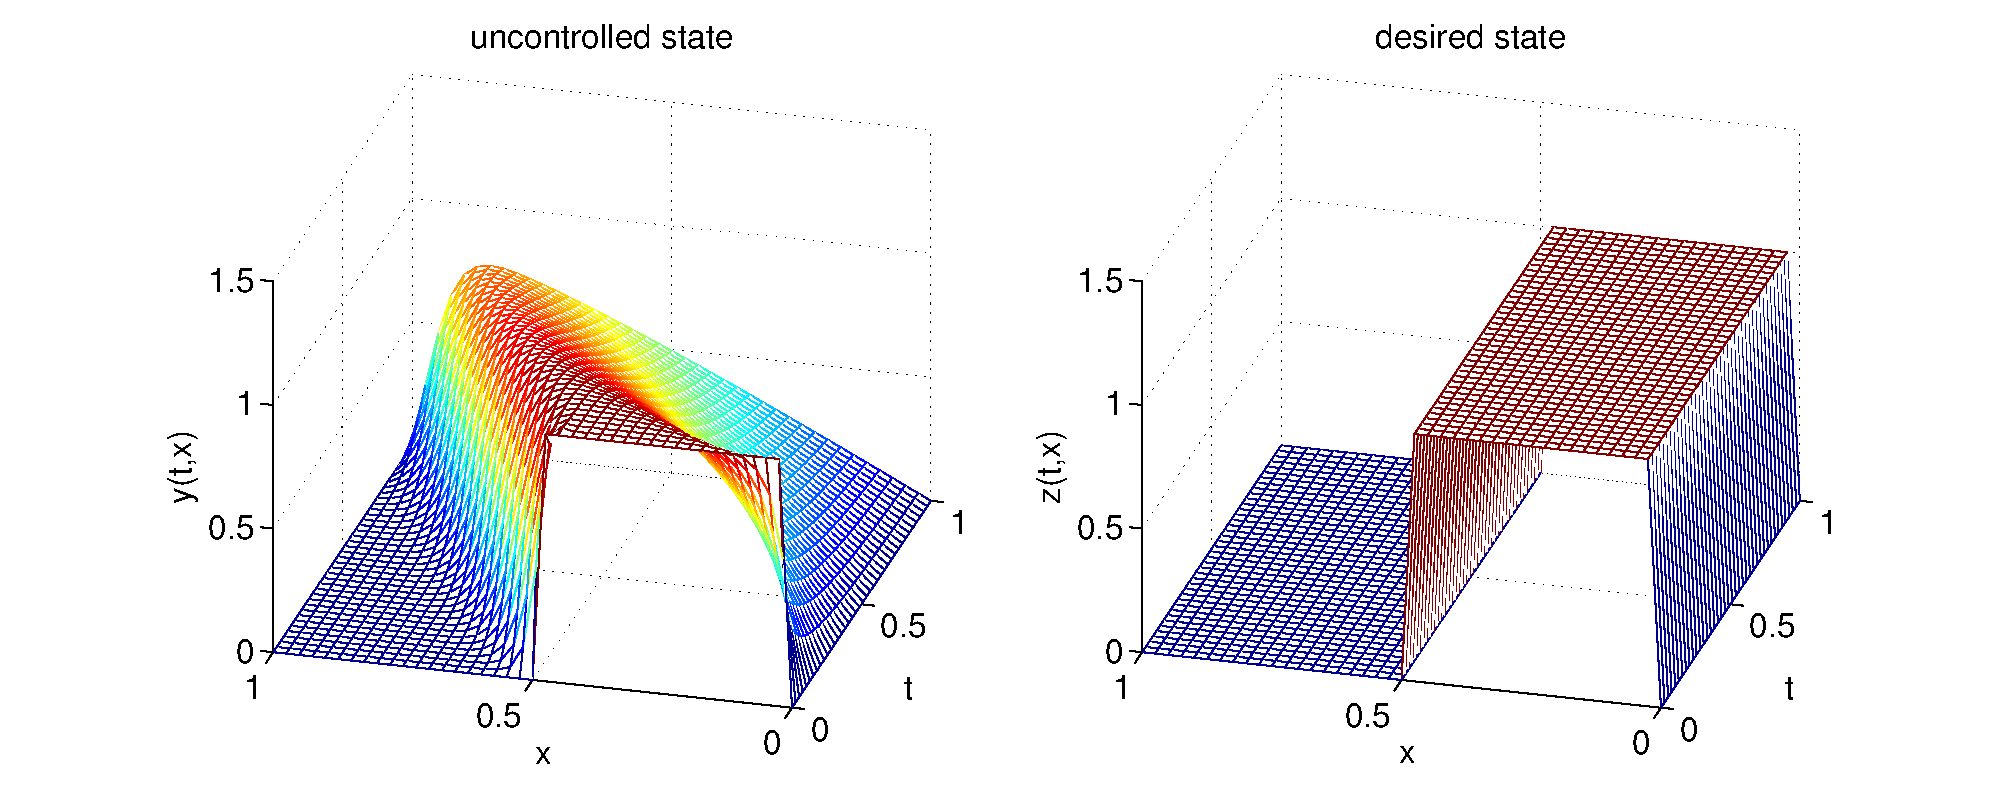
\includegraphics[width=0.9\textwidth]{plots/desiredState}
\caption{Uncontrolled and desired state for $\nu = 0.01$.}\label{desState}
\end{figure}
We now present a discretization of the cost functional \eqref{minJ} as well as Burgers' equation \eqref{Burgers2} which is again in conservative form as already seen in Section \ref{BurgersPODDEIM}. Therefore, we make the ansatz that the control $u$ can be approximated in a finite element way as the superposition of piecewise linear test functions $\phi_j$ as introduced in Appendix \ref{FEMDiscr_space}. This approach can be written as,
\begin{align}
 \label{ansatzu}
 u(t,x) \approx \sum_{j=1}^N u_j(t) \phi_j(x),
\end{align}
where $u_j$ are the respective coefficients of $\phi_j$ that only depend on time, see for example \cite{FEMbook}. Note, that this ansatz also implies that the control is zero at the boundary of $\Omega$ and, therefore, does not change the behavior of the solution $y$ at those points. Furthermore, we will choose $u(0,x) = 0$ as initial control which, again, does not affect the initial condition on $y$.

In order to discretize \eqref{minJ}, the outermost time integral has been approximated by a simple sum using a constant step size $\delta \! t$ for the discretization of the time interval $[0,T]$. We therefore obtain all time-dependent quantities at discrete time instances $t_i$, where $t_0 = 0$ and $t_{N_t} = T$. Recall, that in Appendix \ref{FEMDiscr_space} the state has been approximated in the following way, $y(t,x) \approx \sum_{j=1}^N y_j(t) \phi_j(x)$, a fully discrete version of the cost functional is given by,
\begin{align}
\label{minJ_discr}
\min_{\mathbf{u}_0,...,\mathbf{u}_{N_t}} \mathcal{J}(\mathbf{y}_0,...,\mathbf{y}_{N_t},\mathbf{u}_0,...,\mathbf{u}_{N_t}) = \min_{\mathbf{u}_0,...,\mathbf{u}_{N_t}} \sum_{i=0}^{N_t} \delta \! t \left(\frac{1}{2}\mathbf{y}_i^T M \mathbf{y}_i - \mathbf{z}^T \mathbf{y}_i + \frac{\omega}{2} \mathbf{u}_i^T M \mathbf{u}_i  \right),
\end{align}
where the vector-valued quantities
\begin{align*}
\mathbf{y}_i = \begin{pmatrix}y_1(t_i) \\ \vdots \\ y_N(t_i) \end{pmatrix} \in \mathbb{R}^N, \quad \mathbf{u}_i = \begin{pmatrix}u_1(t_i) \\ \vdots \\ u_N(t_i) \end{pmatrix} \in \mathbb{R}^N, \quad \text{ for }t_i \in [0,T]
\end{align*}
are introduced and $M$ is the mass matrix as defined in Appendix \ref{FEMDiscr_space}. Note, that in \eqref{minJ_discr} the constant and positive term
\begin{align*}
\frac{1}{2} \int_0^T \int_0^L z^2(t,x) \ dx \ dt
\end{align*}
has been neglected since it does not influence the position of the minimum with respect to $u$. This can lead to a negative value of the discrete objective function even though \eqref{minJ} is positive. Furthermore, we assume that the desired state $z$ does not depend on time. The vector $\mathbf{z}$ tested against the hat functions $\phi_j$ is therefore given by,
\begin{align}
\label{fullz}
\mathbf{z} = \begin{pmatrix} \int_0^L z(x) \phi_1(x) dx \\ \vdots \\ \int_0^L z(x) \phi_N(x) dx\\ \end{pmatrix} \approx h \begin{pmatrix} z(x_1) \\ \vdots \\ z(x_N)\\ \end{pmatrix}.
\end{align}
The discretization of Burgers' equation \eqref{Burgers2} with the control on the right-hand side has been obtained by a finite element approach in space and an implicit Euler method in time as described in Appendix \ref{FEMDiscr_space} and Appendix \ref{implEuler}, respectively. The resulting discrete constraint in the form $c(y,u) = 0$ is a vector-valued function with the components equal to,
\begin{align}
\label{Burgers2_discr}
c_{i+1}(\mathbf{y}_i,\mathbf{y}_{i+1},\mathbf{u}_{i+1}) \equiv \frac{1}{\delta \! t} M \mathbf{y}_{i+1} - \frac{1}{\delta \! t} M \mathbf{y}_i + \frac{1}{2} B \mathbf{y}_{i+1}^2 + \nu C \mathbf{y}_{i+1} - \mathbf{f} - M \mathbf{u}_{i+1} = 0,
\end{align}
where $i=0,...,N_t-1$ and the constraint is given by $c := [c_1,...,c_{N_t}]^T$ which is a function of the state and the control at all discrete time instances.

Note, that the only nonlinearity that remains is derived from the discretization of the convective term of Burgers' equation. We will denote this nonlinearity by,
\begin{align}
 \label{fullNonlin}
 \mathcal{N}(\mathbf{y}_{i+1}) := \frac{1}{2} B \mathbf{y}_{i+1}^2,
\end{align}
and point out the special treatment of the nonlinearity in the following application of the Newton-type method using adjoint techniques for the derivative computation as introduced in Section \ref{optAdj}.

Therefore, we first note that after discretization in space and time, the cost function \eqref{minJ_discr} together with the constraint \eqref{Burgers2_discr} fit the framework of \eqref{allgControl}. We can, thus, build the fully discretized Lagrangian function according to the definition \eqref{genLagr}. The discrete Lagrangian of the full-order model is given by,
\begin{align}
\label{discLag}
&\mathcal{L}(\mathbf{y}_0,...,\mathbf{y}_{N_t}, \mathbf{u}_0,...,\mathbf{u}_{N_t},\boldsymbol{\lambda}_1,...,\boldsymbol{\lambda}_{N_t}) \nonumber \\
&\ = \sum_{i=0}^{N_t} \delta \! t \left( \frac{1}{2} \mathbf{y}_i^T M \mathbf{y}_i - \mathbf{z}^T\mathbf{y}_i + \frac{\omega}{2} \mathbf{u}_i^T M \mathbf{u}_i \right) \nonumber \\
&\quad +  \sum_{i=0}^{N_t-1} \boldsymbol{\lambda}_{i+1}^T \left( \frac{1}{\delta \! t} M \mathbf{y}_{i+1} - \frac{1}{\delta \! t} M \mathbf{y}_i + \frac{1}{2} B \mathbf{y}_{i+1}^2 + \nu C \mathbf{y}_{i+1} - \mathbf{f} - M \mathbf{u}_{i+1}  \right),
\end{align}
where the adjoint variable $\boldsymbol{\lambda}_i$ at each time instance is a vector of dimension $N$.

In all our numerical test calculations, adjoints were used for the computation of gradients and Hessian-vector products. Therefore, we will next present how the adjoint Algorithms \ref{alg:Adj1} and \ref{alg:Adj2} have been applied to the discretized Burgers' equation \eqref{minJ_discr}-\eqref{Burgers2_discr}.
\subsection{Numerical results for a Newton-type method using adjoints}
\label{NumTests_Hess}
We want to apply the optimization Algorithm \ref{alg:Opt} in order to solve \eqref{minJ_discr} for $\mathbf{u}_0,...,\mathbf{u}_{N_t}$, when $\mathbf{y}_0,...,\mathbf{y}_{N_t}$ is the solution of \eqref{Burgers2_discr}. Therefore, we will need the corresponding Lagrangian function \eqref{discLag} as well as the gradient and the Hessian-times-vector product as described in the algorithms \ref{alg:Adj1} and \ref{alg:Adj2}, respectively. We will concentrate on the solution of the two adjoint equations and refer to Appendix \ref{FEMDiscr} for the numerical solution of Burgers' equation.

In the adjoint Algorithm \ref{alg:Adj1} that computes the gradient of the cost functional \eqref{minJ_discr}, we mostly need to compute partial derivatives of the constraint \eqref{Burgers2_discr} and the cost functional itself with respect to the control $u$ and the state variable $y$. Since both the constraint and the cost functional depend on the control and the state at all time instances, the respective variables we need to consider are of the size $N \cdot N_t$,
\begin{align*}
\mathbf{\underline u} := \begin{pmatrix} \mathbf{u}_0 \\ \vdots \\ \mathbf{u}_{N_t} \end{pmatrix} \in \mathbb{R}^{(N \cdot N_t) \times 1}, \quad \mathbf{\underline y} := \begin{pmatrix} \mathbf{y}_0 \\ \vdots \\ \mathbf{y}_{N_t} \end{pmatrix} \in \mathbb{R}^{(N \cdot N_t) \times 1}.
\end{align*}
Therefore, at every outer iteration of the optimization loop, we first need to solve Burgers' equation on the whole time interval. In Algorithm \ref{alg:Adj1_Burgers}, we summarize the application of Algorithm \ref{alg:Adj1} to the full-order discrete optimal control problem with Burgers' equation as an implicit constraint. Thereby, the adjoint equation \eqref{adjoint1} reduces to an ordinary differential equation in the adjoint variable. Note, that we first need to solve the terminal condition \eqref{AdjFullOrder_term} for $\boldsymbol{\lambda}_{N_t}$ and then solve the set of equations \eqref{AdjFullOrder} backwards in time. Given the solution of \eqref{AdjFullOrder_term}-\eqref{AdjFullOrder}, the gradient of the cost function with respect to the control $u$ can be obtained according to \eqref{grad}.
\begin{algorithm}[H]
\caption{Algorithm \ref{alg:Adj1} applied to the full-order discrete Burgers' equation}
\label{alg:Adj1_Burgers}
\begin{algorithmic}[1]
\STATE From the initial condition $\mathbf{y}_0$ and the current control $\mathbf{u}_1,...,\mathbf{u}_{N_t}$, solve Burgers' equation for $\mathbf{y}_1,...,\mathbf{y}_{N_t}$ as described in Appendix \ref{FEMDiscr}
\STATE The adjoint equation \eqref{adjoint1} reads:
\begin{subequations}
\begin{align}
\label{AdjFullOrder_term}
\left(\frac{1}{\delta \! t}M + \mathcal{N}'(\mathbf{y}_{N_t}) +  \nu C\right)^T \boldsymbol{\lambda}_{N_t} &= -\delta \! t( M \mathbf{y}_{N_t} - \mathbf{ z} )\\
\label{AdjFullOrder}
\left(\frac{1}{\delta \! t}M + \mathcal{N}'(\mathbf{y}_{i}) + \nu C\right)^T \boldsymbol{\lambda}_i &= - (-\frac{1}{\delta \! t} M)^T \boldsymbol{\lambda}_{i+1} -\delta \! t( M \mathbf{y}_{i} - \mathbf{ z} ), \quad i = N_t-1,...,1
\end{align}
\end{subequations}
\STATE The gradient is computed according to formula \eqref{grad}:
\begin{align}
\label{gradFullOrder}
\nabla_u \hat{\mathcal J}(\mathbf{u}_0,...,\mathbf{u}_{N_t}) = \begin{pmatrix} \delta \! t \omega M \mathbf{u}_0 \\ \delta \! t \omega M \mathbf{u}_1 - M^T \boldsymbol{\lambda}_1 \\ \vdots \\ \delta \! t \omega M \mathbf{u}_{N_t} - M^T \boldsymbol{\lambda}_{N_t} \end{pmatrix}
\end{align}
\end{algorithmic}
\end{algorithm}
In \eqref{AdjFullOrder_term} and \eqref{AdjFullOrder} it is necessary to compute the first derivative of the nonlinear term \eqref{fullNonlin}. For an arbitrary vector $\mathbf{y} = [y_1,...,y_N]^T$ and a matrix $B \in \mathbb{R}^{N \times N}$, the first derivative of the nonlinear term $\mathcal{N}(\cdot)$ is given by,
\begin{align*}
\mathcal{N}'(\mathbf{y}) = \frac{d}{d\mathbf{y}}\left( \frac{1}{2} B \mathbf{y}^2 \right) = \begin{pmatrix} B_{1,1}y_1 & \hdots & B_{1,N}y_N \\
                                   B_{2,1}y_1 & \hdots & B_{2,N}y_N \\
                                      \vdots  &        &     \vdots \\
                                   B_{N,1}y_1 & \hdots & B_{N,N}y_N \end{pmatrix} \in \mathbb{R}^{N \times N},
\end{align*}
which is again an $N \times N$ matrix.

In order to solve the Newton equation \eqref{Newtoneqn_J} we also need to compute the Hessian $\nabla^2 \hat{\mathcal J}(u)$. Since this is a matrix of dimension $N \cdot N_t \times N \cdot N_t$, we solve the linear system \eqref{Newtoneqn_J} with the truncated CG method where we only need to compute the product of the Hessian times a vector and never need to store the whole Hessian matrix, see Algorithm \ref{alg:serCG}. In Algorithm \ref{alg:Adj2_Burgers}, we present the application of the general Hessian-times-vector computation as derived in Section \ref{Hessadj} to the optimization of Burgers' equation. Therefore, we define the arbitrary vector $\mathbf{\underline v} := (\mathbf{v}^T_0, ..., \mathbf{v}^T_{N_t} )^T$ and derive the equations \eqref{wFullOrder_init}-\eqref{wFullOrder} and \eqref{pFullOrder_term}-\eqref{pFullOrder} for the auxiliary variables $w$ and $p$ according to the respective general formulas \eqref{eqnw} and \eqref{eqnp}. It is important to note that the initial condition \eqref{wFullOrder_init} and the terminal condition \eqref{pFullOrder_term} follow directly from the general equations \eqref{eqnw} and \eqref{eqnp} when the respective partial derivative is computed.
\newpage
\begin{algorithm}[H]
\caption{Algorithm \ref{alg:Adj2} applied to the full-order discrete Burgers' equation}
\label{alg:Adj2_Burgers}
\begin{algorithmic}[1]
\STATE We assume that we have already computed $\mathbf{y}_0,...,\mathbf{y}_{N_t}, \mathbf{u}_0,...,\mathbf{u}_{N_t},\boldsymbol{\lambda}_1,...,\boldsymbol{\lambda}_{N_t}$ in \mbox{Algorithm \ref{alg:Adj1_Burgers}}
\STATE Equation \eqref{eqnw} reads:
\begin{subequations}
\begin{align}
\label{wFullOrder_init}
\mathbf{w}_0 &= 0 \\
\label{wFullOrder}
\left( \frac{1}{\delta \! t}M + \mathcal{N}'(\mathbf{y}_{i+1}) + \nu C \right) \mathbf{w}_{i+1} &= - (-\frac{1}{\delta \! t} M) \mathbf{w}_i - M\mathbf{v}_{i+1} , \quad i = 0,...,N_t-1
\end{align}
\end{subequations}
\STATE Equation \eqref{eqnp} reads:
\begin{subequations}
\begin{align}
\label{pFullOrder_term}
\left( \frac{1}{\delta \! t}M + \mathcal{N}'(\mathbf{y}_{N_t}) + \nu C \right)^T \mathbf{p}_{N_t} &= \delta \! t M \mathbf{w}_{N_t} + \text{diag}(\boldsymbol{\lambda}^T_{N_t} b_1,...,\boldsymbol{\lambda}^T_{N_t} b_N) \mathbf{w}_{N_t}\\
\label{pFullOrder}
\left( \frac{1}{\delta \! t}M + \mathcal{N}'(\mathbf{y}_{i}) + \nu C \right)^T \mathbf{p}_{i} &= - (-\frac{1}{\delta \! t} M)^T \mathbf{p}_{i+1} + \delta \! t M \mathbf{w}_{i} \nonumber \\
&\quad + \text{diag}(\boldsymbol{\lambda}^T_{i} b_1,...,\boldsymbol{\lambda}^T_{i} b_N) \mathbf{w}_{i}, \quad i = N_t-1,...,1
\end{align}
\end{subequations}
\STATE The Hessian times a vector $\mathbf{\underline v}$ is computed according to formula \eqref{hesseqn}:
\begin{align}
\label{HessFullOrder}
\nabla^2 \hat{\mathcal J}(\mathbf{u}_0,...,\mathbf{u}_{N_t}) \cdot \mathbf{\underline v} = \begin{pmatrix} \delta \! t \omega M \mathbf{v}_0 \\ -M^T \mathbf{p}_1 + \delta \! t \omega M \mathbf{v}_1\\ \vdots \\ -M^T \mathbf{p}_{N_t} + \delta \! t \omega M \mathbf{v}_{N_t} \end{pmatrix}
\end{align}
\end{algorithmic}
\end{algorithm}
Note that in \eqref{pFullOrder_term}-\eqref{pFullOrder} as well as in \eqref{HessFullOrder} it is necessary to compute second partial derivatives of the Lagrangian function. Therefore, we first note that due to the definition of the Lagrangian, mixed second order derivatives vanish. Furthermore, we present the analytic computation of the second partial derivative of the quantity $\boldsymbol{\lambda}^T \mathcal{N}(\mathbf{y})$ with respect to the state variable $\mathbf{y}$,
\begin{align*}
\frac{d^2}{d\mathbf{y}^2} \left( \boldsymbol{\lambda}^T \mathcal{N}(\mathbf{y}) \right) \mathbf{w} &= \frac{d^2}{d\mathbf{y}^2} \left( \boldsymbol{\lambda}^T (\frac{1}{2} B \mathbf{y}^2) \right) \mathbf{w}
= \frac{d^2}{d\mathbf{y}^2} \left( \frac{1}{2} \sum_{k=1}^N \lambda_k \sum_{j=1}^N B_{k,j}y_j^2 \right) \mathbf{w} \\
&= \frac{d}{d\mathbf{y}}\begin{pmatrix} \sum_{k=1}^N \lambda_k B_{k,1}y_1 \\ \vdots \\ \sum_{k=1}^N \lambda_k B_{k,N}y_N \end{pmatrix} \mathbf{w}
= \begin{pmatrix} \sum_{k=1}^N \lambda_k B_{k,1} & & \\ & \ddots & \\ & & \sum_{k=1}^N \lambda_k B_{k,N}\end{pmatrix}\mathbf{w} \\
&= \text{diag}(\boldsymbol{\lambda}^T b_1,...,\boldsymbol{\lambda}^T b_N) \mathbf{w},
\end{align*}
where $\boldsymbol{\lambda} = (\lambda_1,...,\lambda_N)^T$, $\mathbf{y} = (y_1,..,y_N)^T$ ,and $b_1,...,b_N$ are the columns of the matrix $B$ such that $B = (b_1 |... | b_N)$.

Figures \ref{optFull} and \ref{optFullu} show numerical results of Algorithm \ref{alg:Opt} applied to problem \eqref{minJ_discr} with implicit constraint \eqref{Burgers2_discr}. In the considered setting, we chose $\nu = 0.01$ in Burgers' equation, $\omega = 0.005$ for the control penalty, and $N = N_t = 80$ grid points in time and space. In order to be able to perform the optimization Algorithm \ref{alg:Opt} using Armijo line search as described in Algorithm \ref{alg:Armijo} and the gradient and Hessian-vector product computation in Algorithms \ref{alg:Adj1_Burgers} and \ref{alg:Adj2_Burgers}, respectively, we need to specify some settings which have been summarized in Table \ref{params}. Also the Newton iteration for the numerical solution of Burgers' equation requires to set some tolerances.
\begin{table}[H]
\centering
\begin{tabular}{|c|c|c|c|c|c|c|}
  \hline
  $\varepsilon_\mathcal{J}$ & $\varepsilon_\nabla$ & $\varepsilon_\alpha$ & $\alpha_{min}$ & $\eta_k$ & $\varepsilon_{Newton}$ & \texttt{max\_newton} \\
  \hline
  \texttt{10e-8} & \texttt{10e-9} & \texttt{10e-4} & \texttt{10e-8} & \texttt{10e-2} & \texttt{10e-3} & \texttt{20} \\
  \hline
\end{tabular}
\caption{Choice of parameters for the numerical results in Figure \ref{optFull} and \ref{optFullu}.}\label{params}
\end{table}
The outer optimization loop of algorithm \ref{alg:Opt} stops when either the value of the objective function does not change anymore ($\varepsilon_\mathcal{J}$ in Algorithm \ref{alg:Opt}) or the zero-gradient condition is fulfilled up to a certain precision ($\varepsilon_\nabla$ in Algorithm \ref{alg:Opt}). The tolerance of the Armijo line  search is set by $\varepsilon_\alpha$ and a minimum step length is guaranteed by $\alpha_{min}$, see Algorithm \ref{alg:Armijo}. The truncated CG-algorithm \ref{alg:serCG} is terminated by the choice of $\eta_k$, and $\varepsilon_{Newton}$ and \texttt{max\_newton} are, respectively, the tolerance and the maximum number of iterations of Newton's method as described in Algorithm \ref{alg:Euler}.

From the numerical results in Figure \ref{optFull}, we see that the state variable $y$ converges to the desired state $z$ as the number of optimization iterations $k$ increases. For the presented setting, after $6$ iterations a state has been reached such that the value of the objective function \eqref{minJ_discr} does not decrease any further than \texttt{0.024}.
\begin{figure}[H]
\centering
\subfloat[$k=0$ (uncontrolled)]{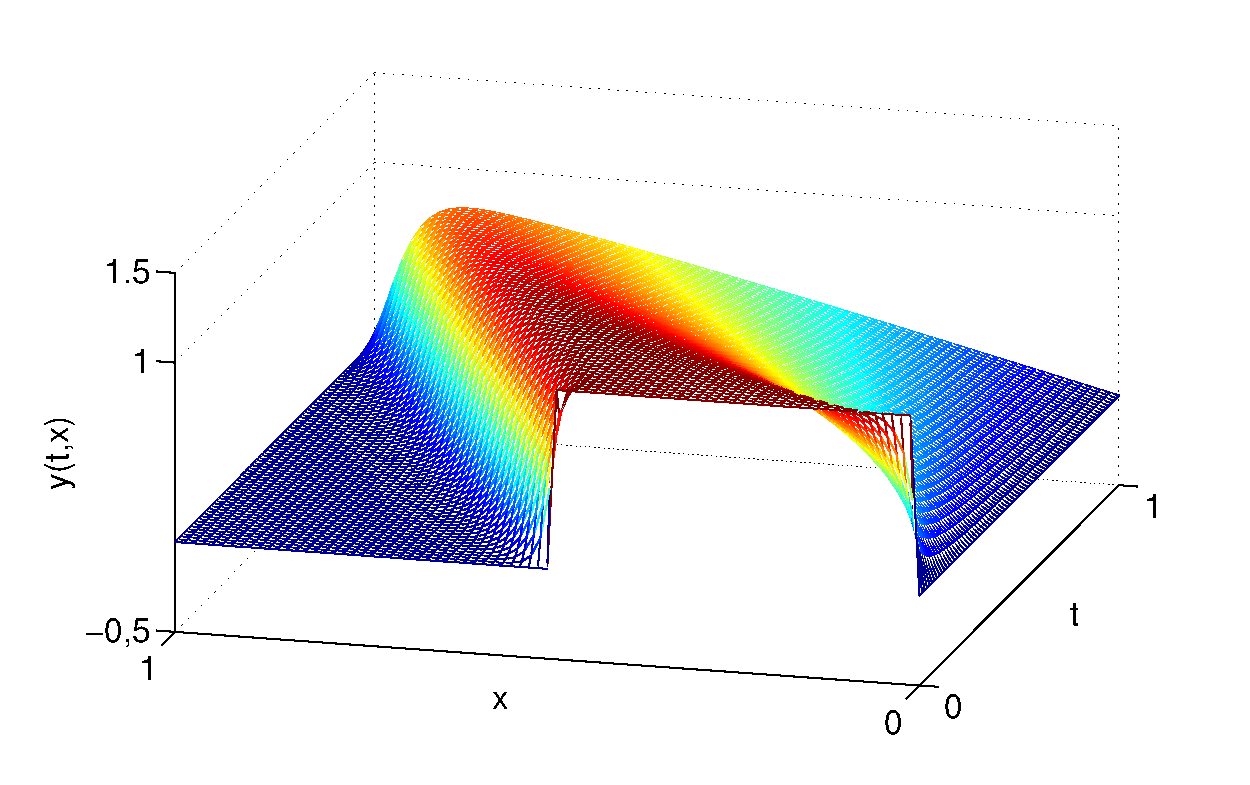
\includegraphics[width=0.33\textwidth]{plots/controlFullk0_new}}\hfill
\subfloat[$k=1$ ]{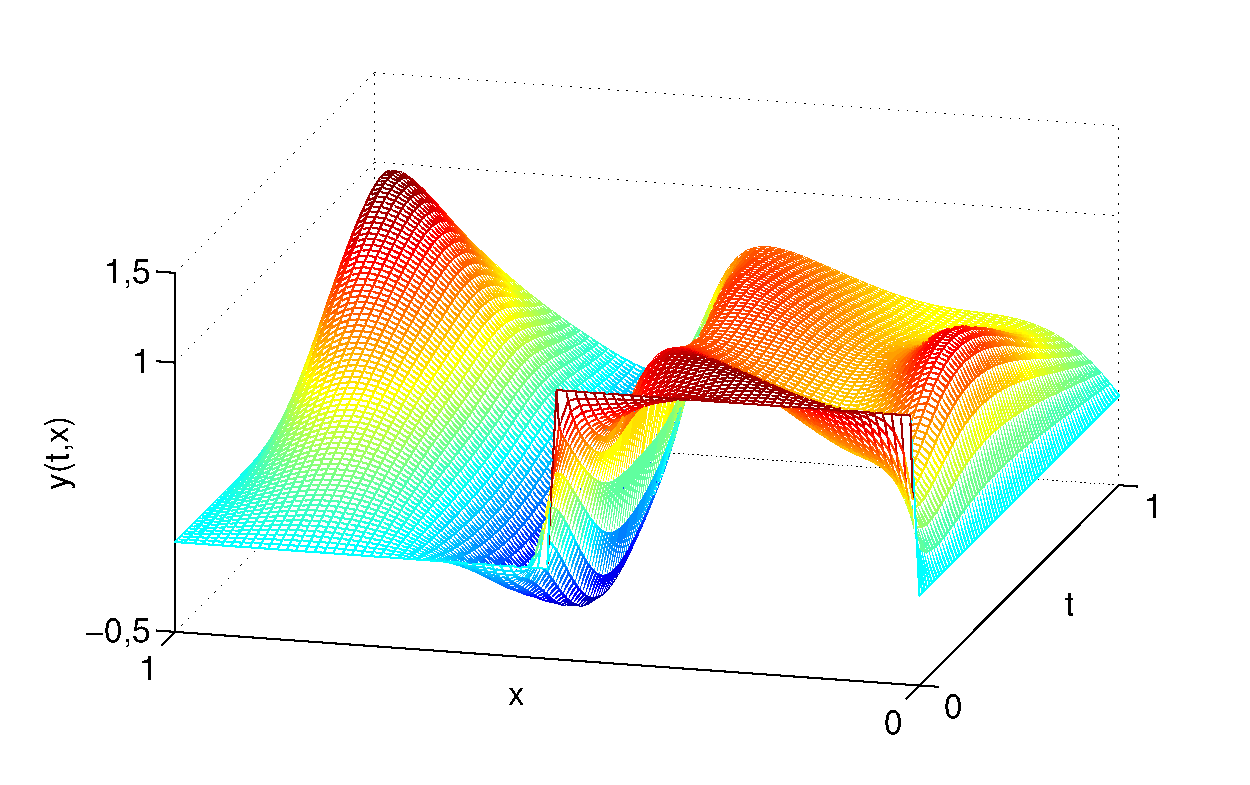
\includegraphics[width=0.33\textwidth]{plots/controlFullk1_new}}\hfill
\subfloat[$k=2$]{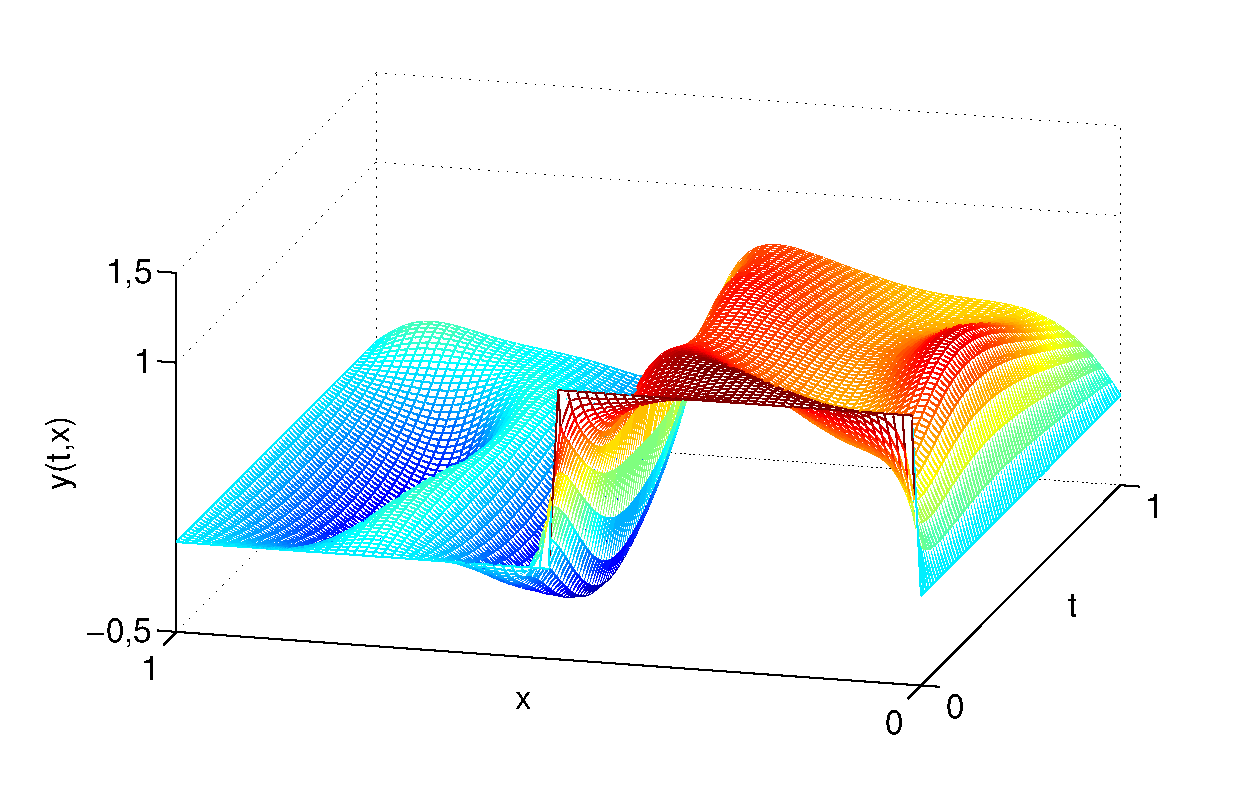
\includegraphics[width=0.33\textwidth]{plots/controlFullk2_new}}\\
\subfloat[$k=3$ ]{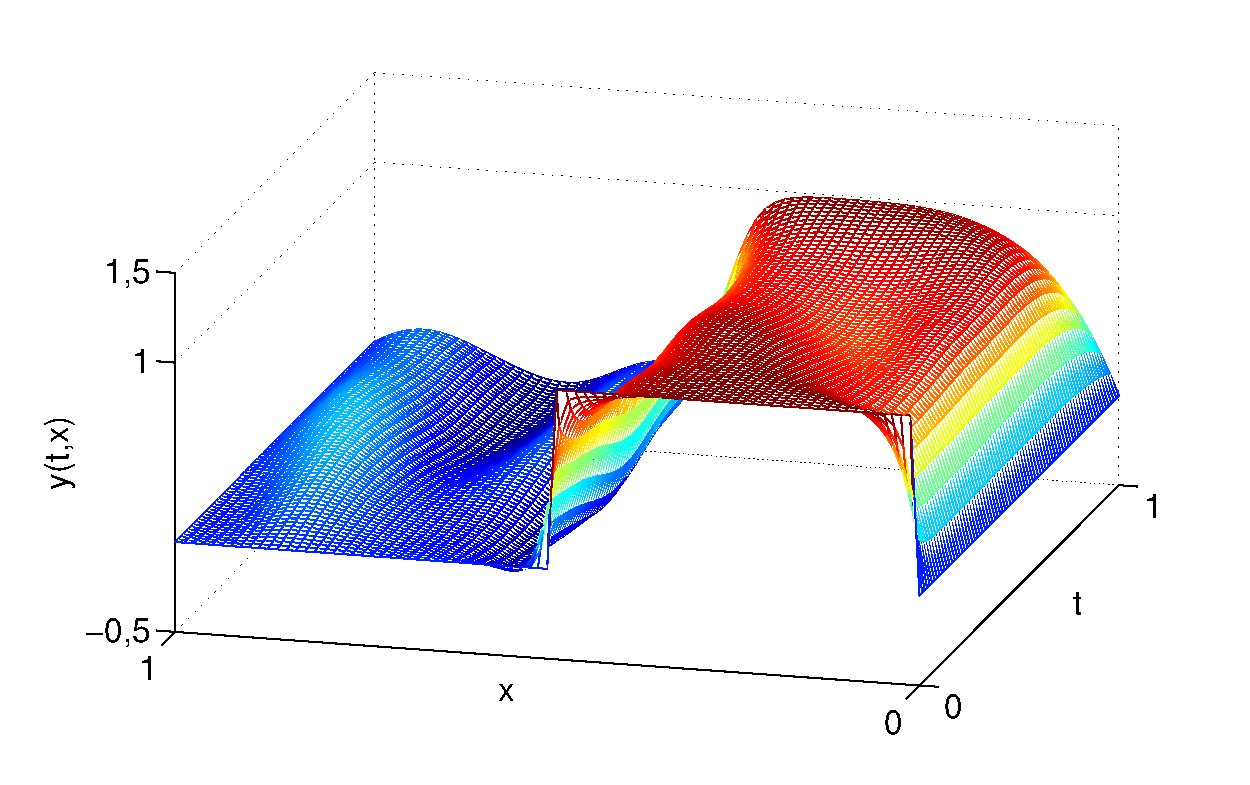
\includegraphics[width=0.33\textwidth]{plots/controlFullk3_new}}\hfill
\subfloat[$k=4$ ]{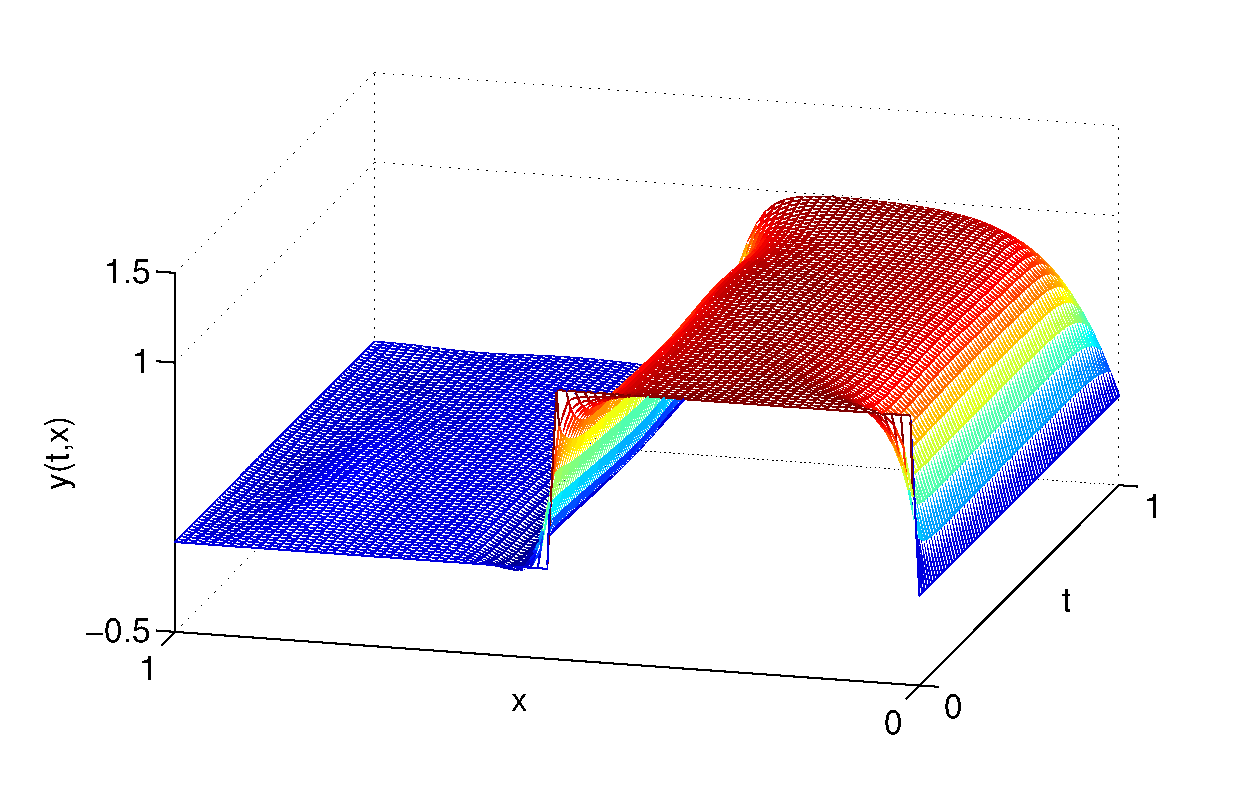
\includegraphics[width=0.33\textwidth]{plots/controlFullk4_new}}\hfill
\subfloat[$k=5$]{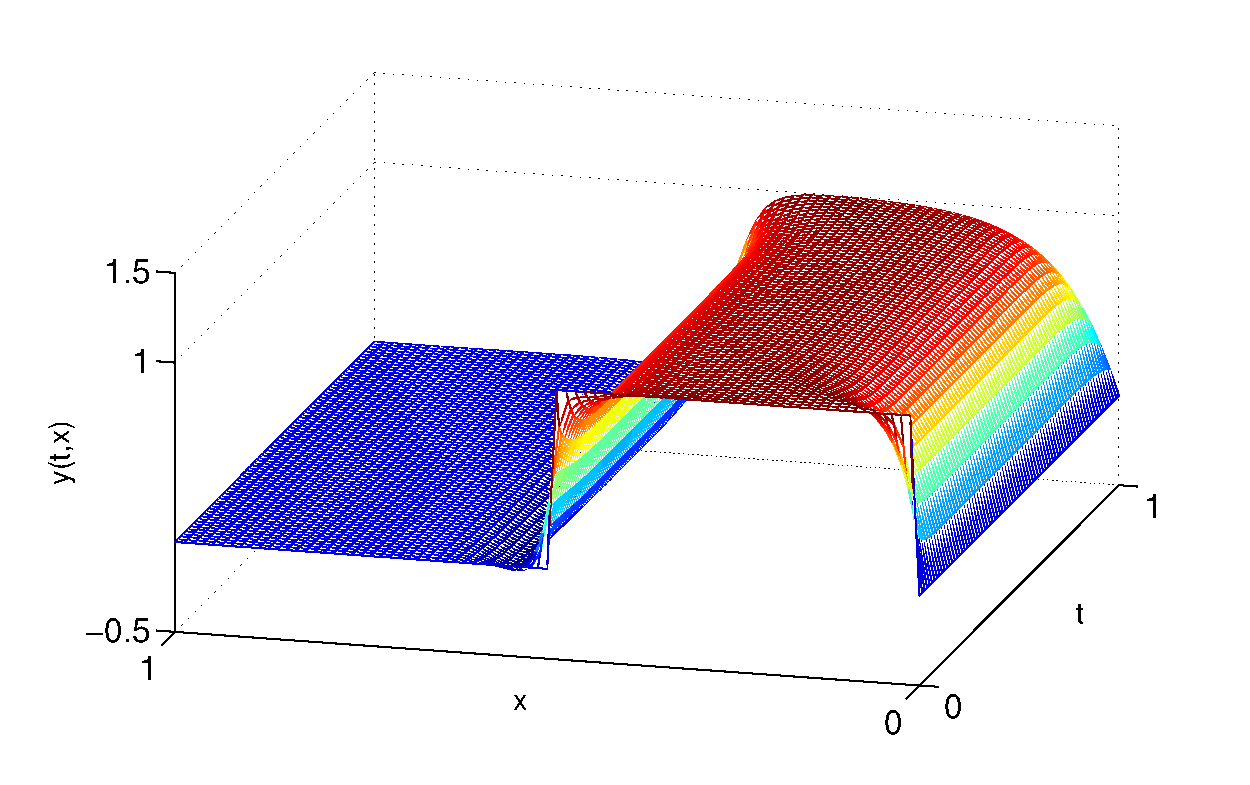
\includegraphics[width=0.33\textwidth]{plots/controlFullk5_new}}\\
\caption{The state $y$ at different stages $k$ of the optimization iteration.}\label{optFull}
\end{figure}
In Figure \ref{optFullu}, we present the control that corresponds to the states presented before. After convergence, we see in the last plot of Figure \ref{optFullu} the desired optimal control $u^*$ that drives the solution to Burgers' equation into the desired state $z$, i.e. minimizes the cost function.
\begin{figure}[H]
\centering
\subfloat[$k=0$ (initial)]{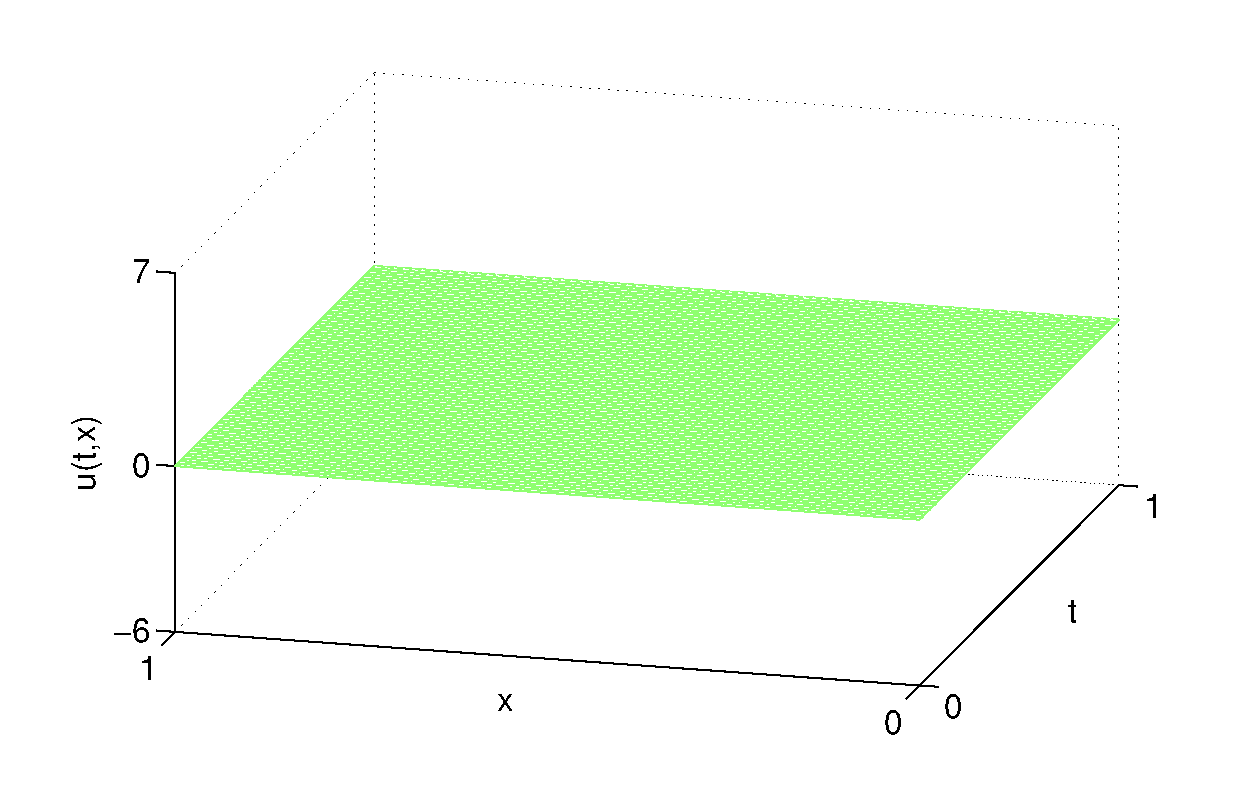
\includegraphics[width=0.33\textwidth]{plots/uFullk0_new}}\hfill
\subfloat[$k=1$ ]{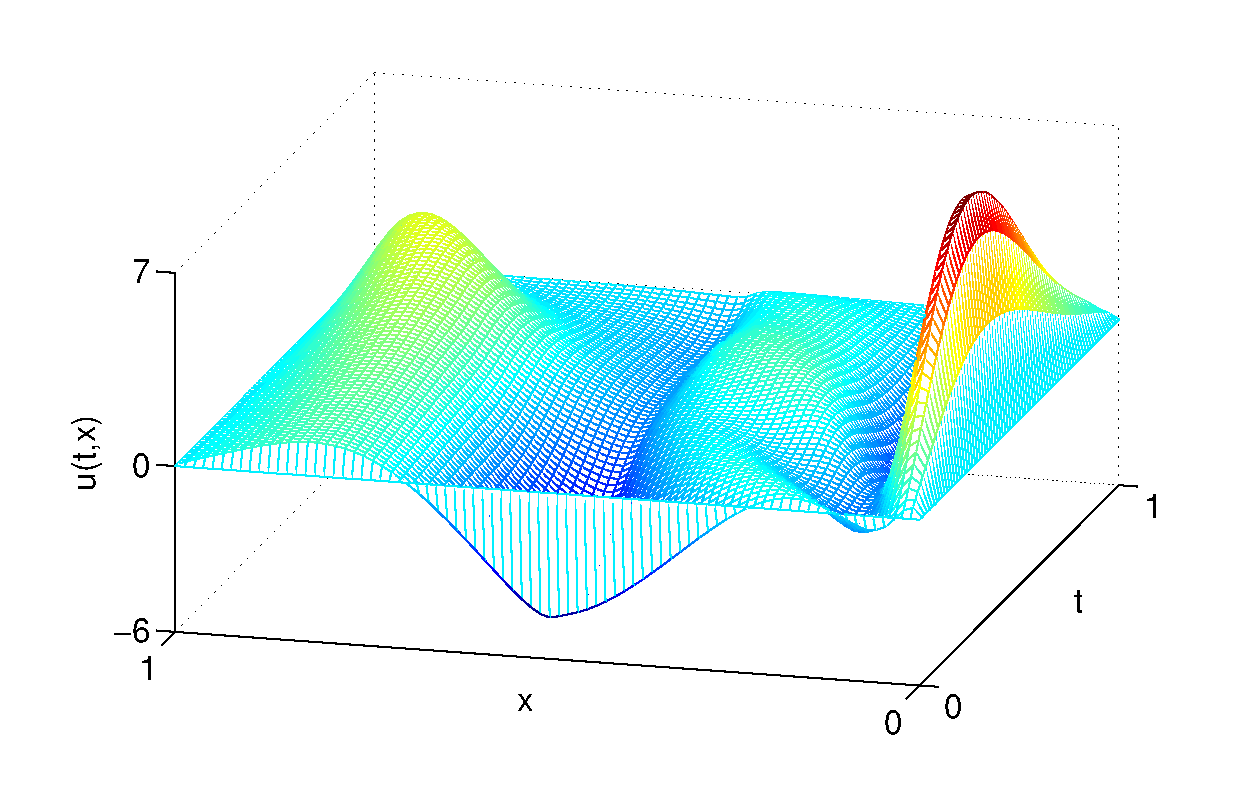
\includegraphics[width=0.33\textwidth]{plots/uFullk1_new}}\hfill
\subfloat[$k=2$]{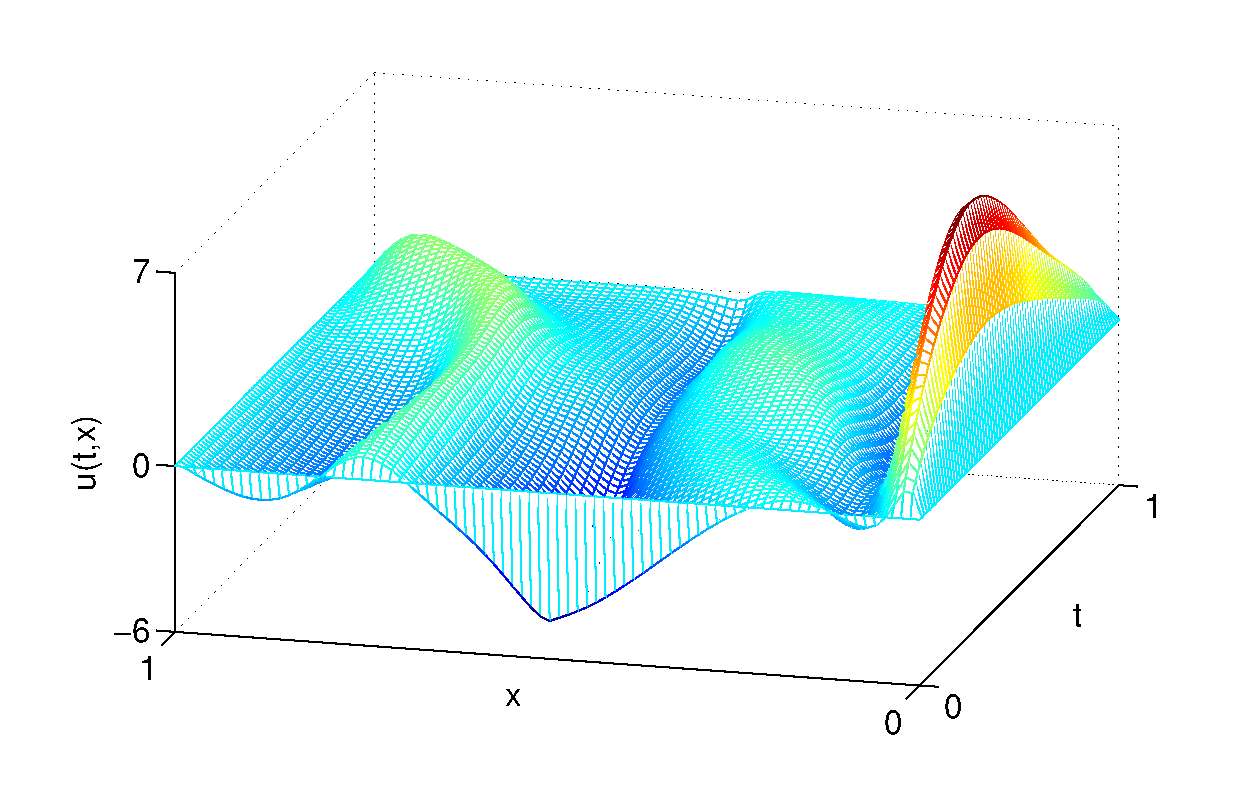
\includegraphics[width=0.33\textwidth]{plots/uFullk2_new}}\\
\subfloat[$k=3$ ]{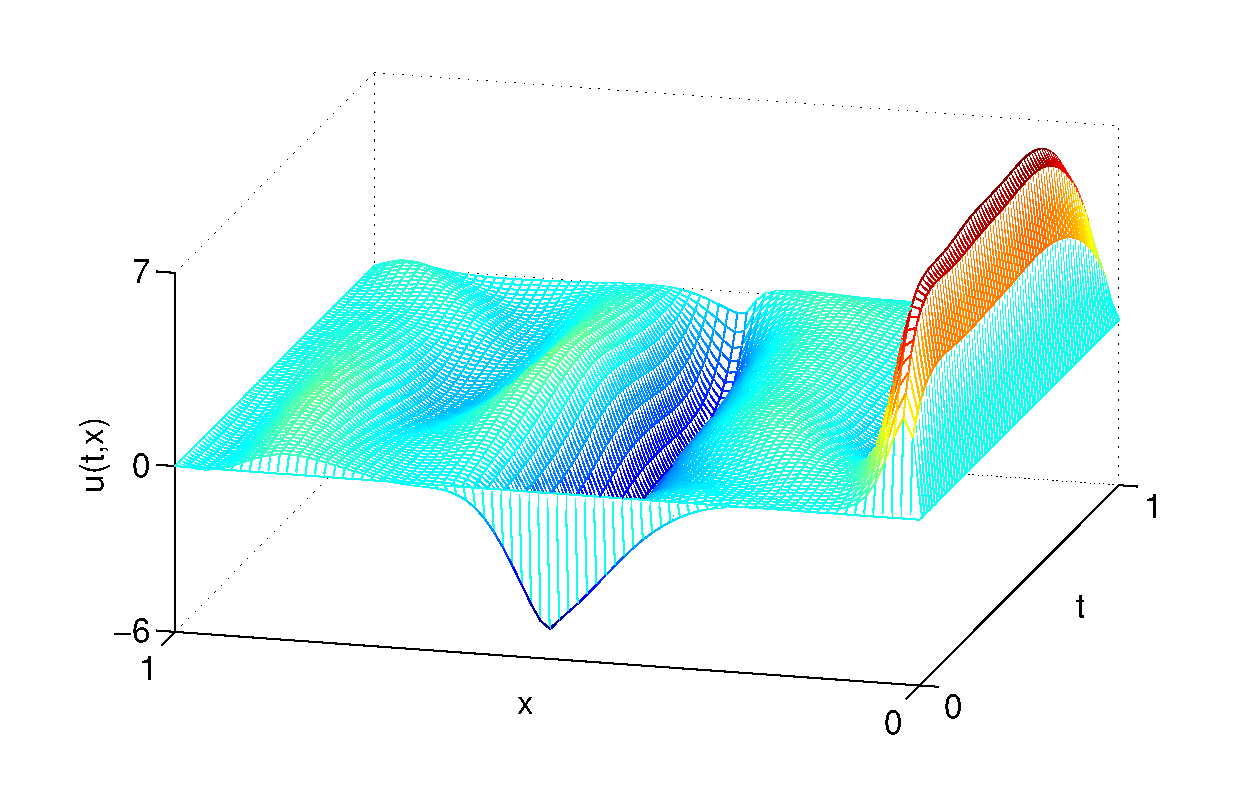
\includegraphics[width=0.33\textwidth]{plots/uFullk3_new}}\hfill
\subfloat[$k=4$ ]{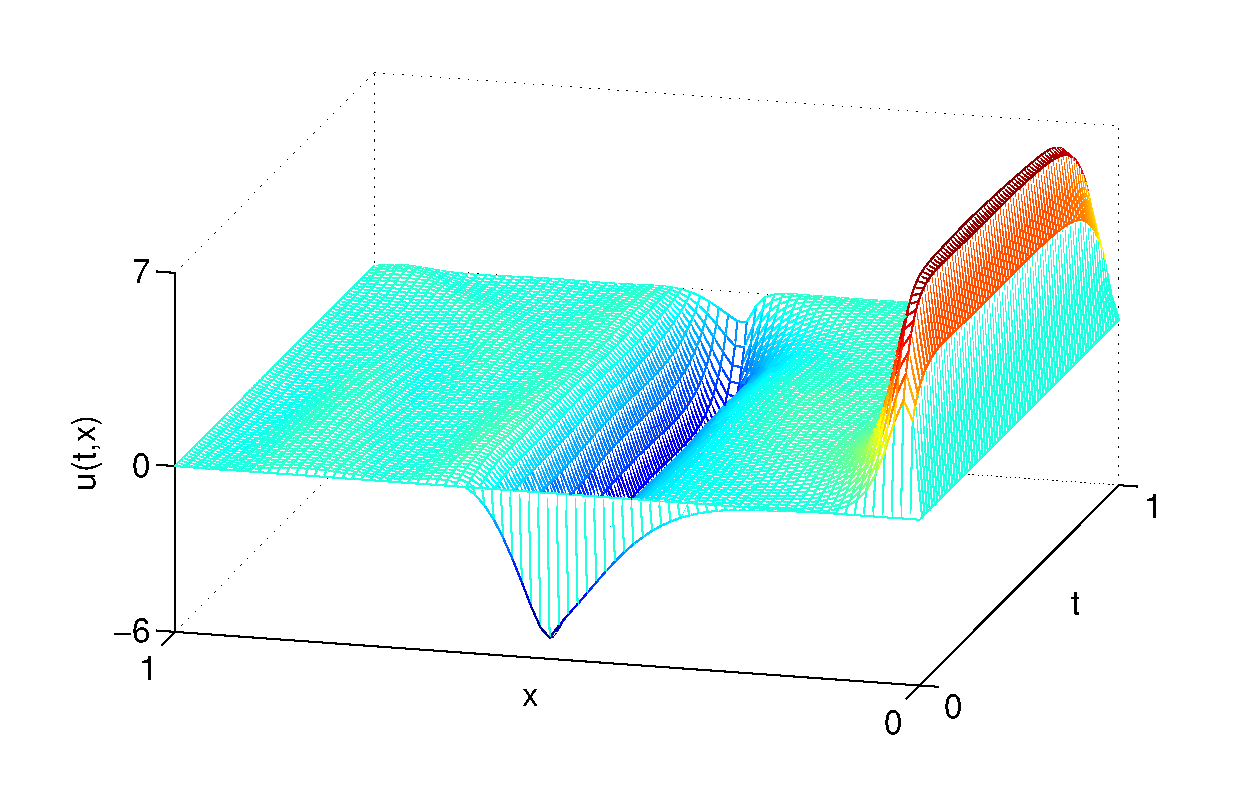
\includegraphics[width=0.33\textwidth]{plots/uFullk4_new}}\hfill
\subfloat[$k=5$]{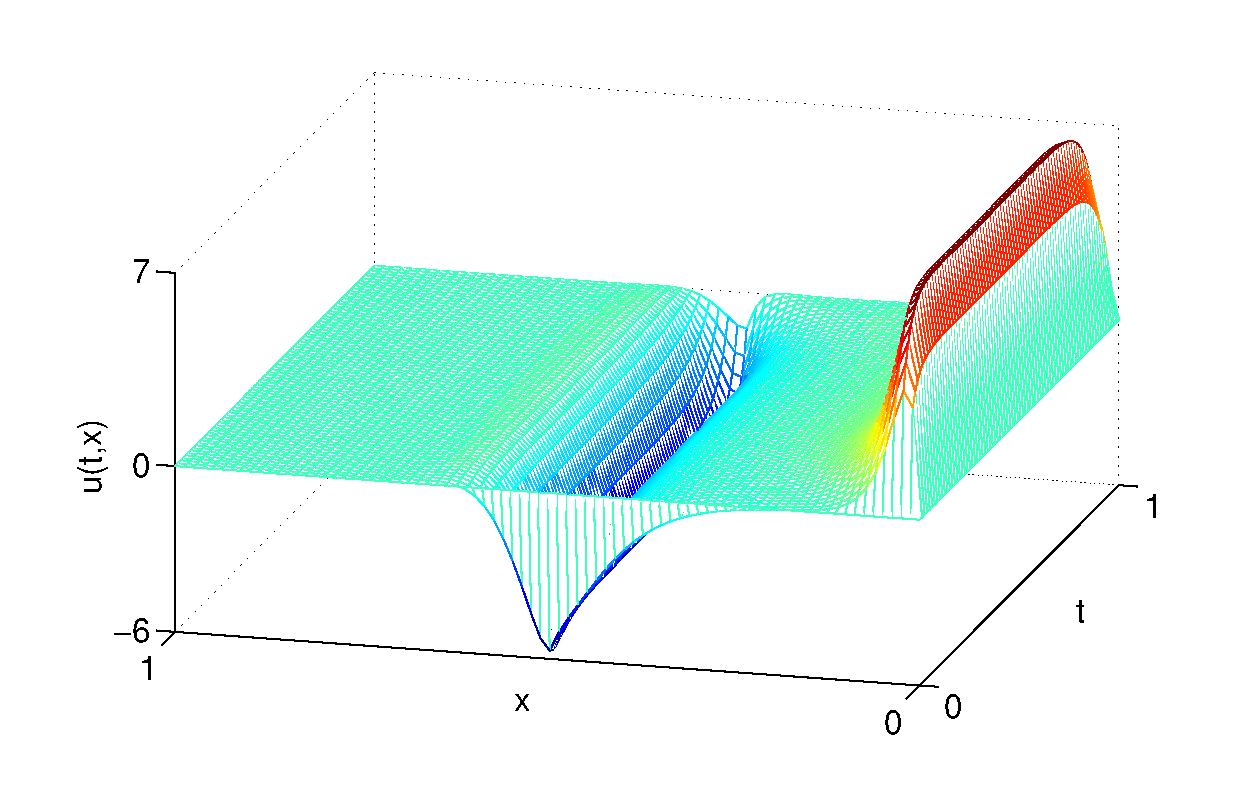
\includegraphics[width=0.33\textwidth]{plots/uFullk5_new}\label{optFullu_opt}}\\
\caption{The control $u$ at different stages $k$ of the optimization iteration.}\label{optFullu}
\end{figure}
A second numerical test using the same parameters as in Table \ref{params} has been performed in order to show the dependence of the optimization algorithm on the control penalty $\omega$. From \eqref{minJ} we see that the smaller we choose $\omega$ the more we put emphasis on driving the state $y$ into the desired state and allow a large control.
\begin{figure}[H]
\centering
\subfloat{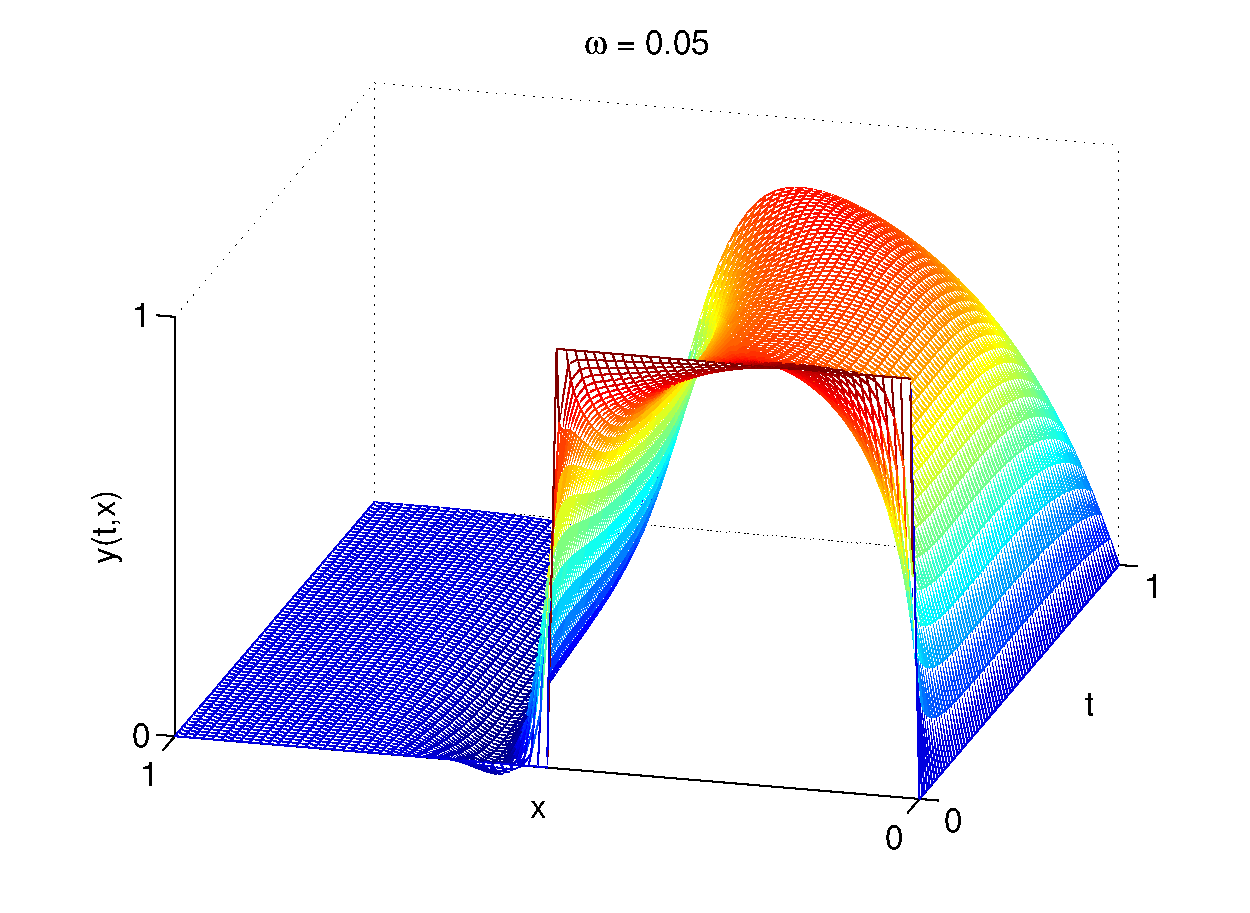
\includegraphics[width=0.33\textwidth]{plots/y_w05}}\hfill
\subfloat{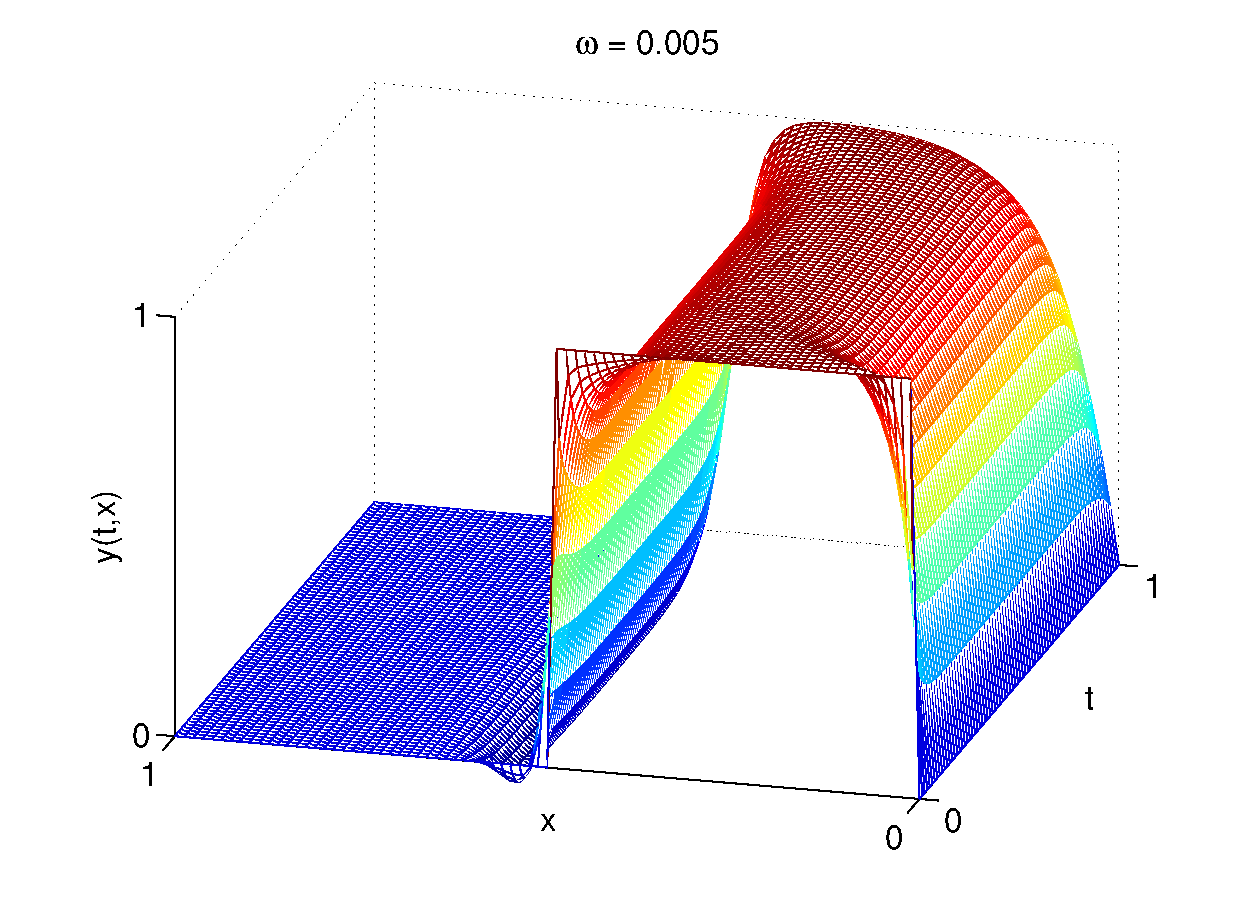
\includegraphics[width=0.33\textwidth]{plots/y_w005}}\hfill
\subfloat{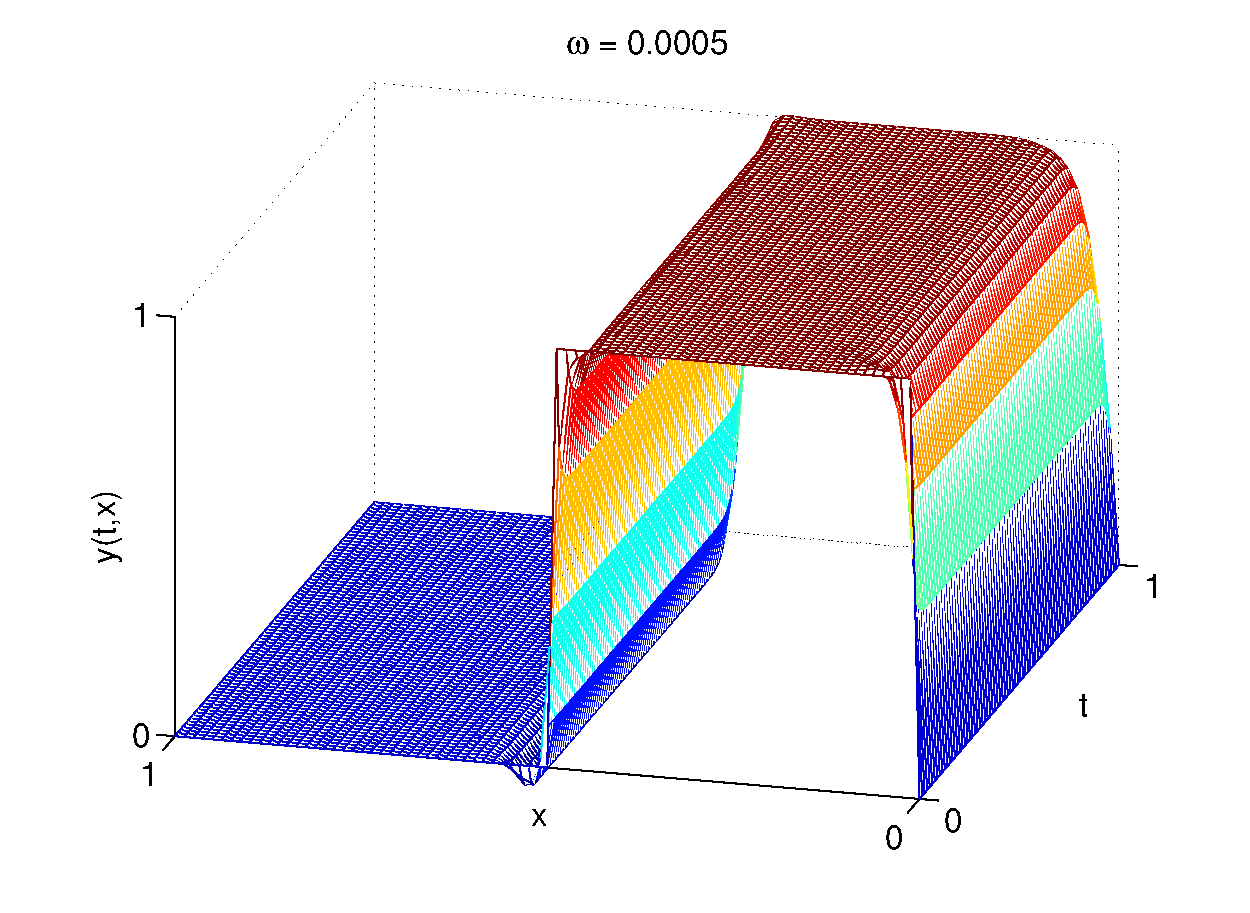
\includegraphics[width=0.33\textwidth]{plots/y_w0005}}\\
\subfloat{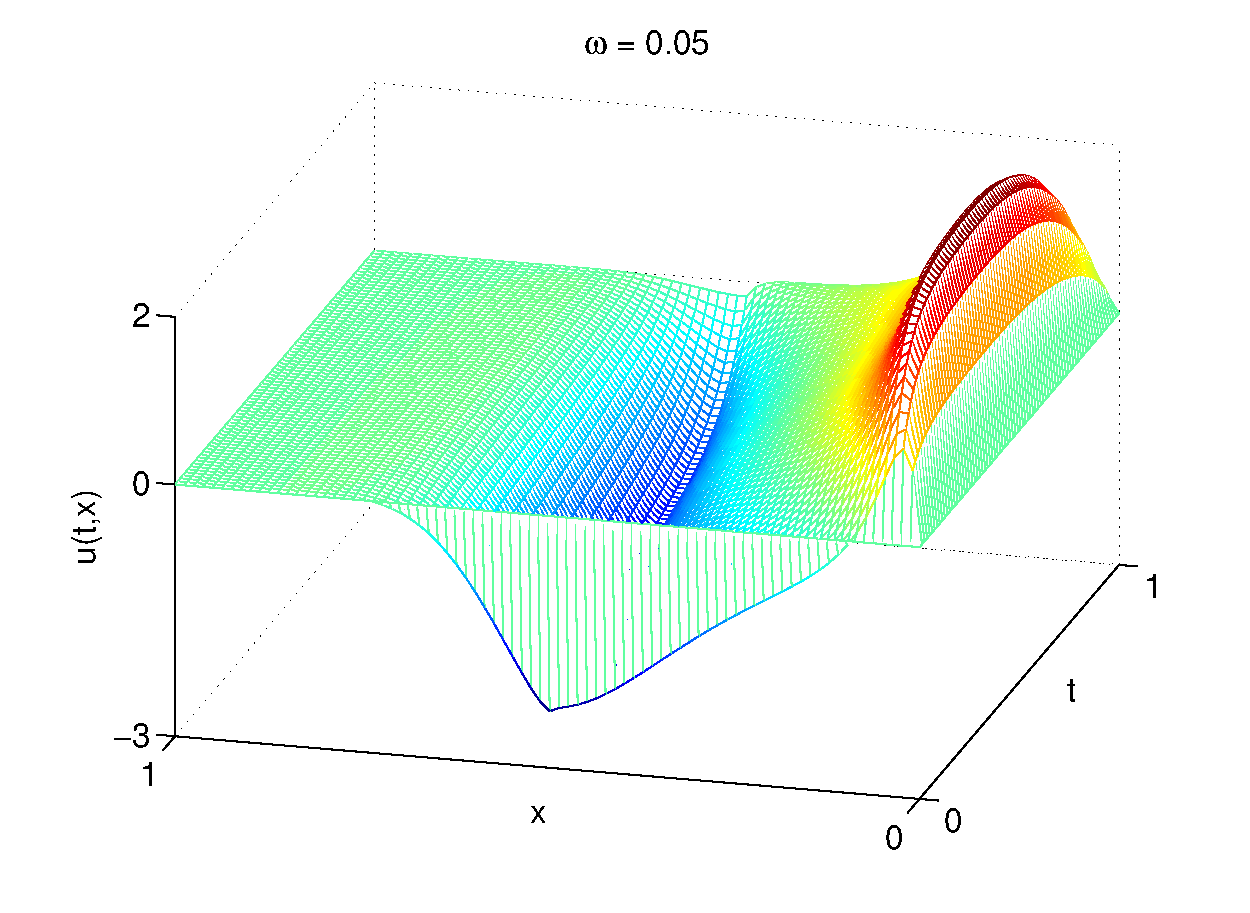
\includegraphics[width=0.33\textwidth]{plots/u_w05}}\hfill
\subfloat{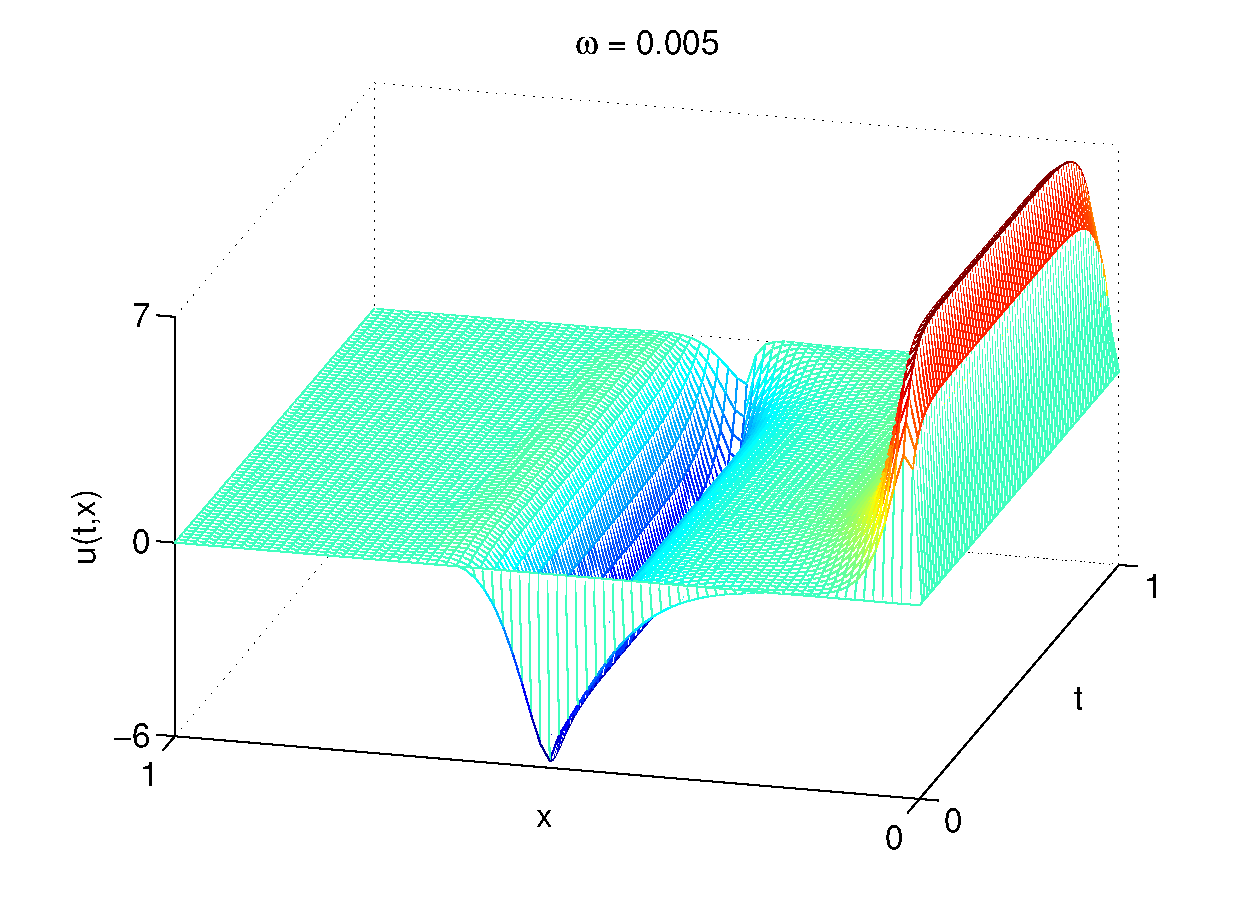
\includegraphics[width=0.33\textwidth]{plots/u_w005}}\hfill
\subfloat{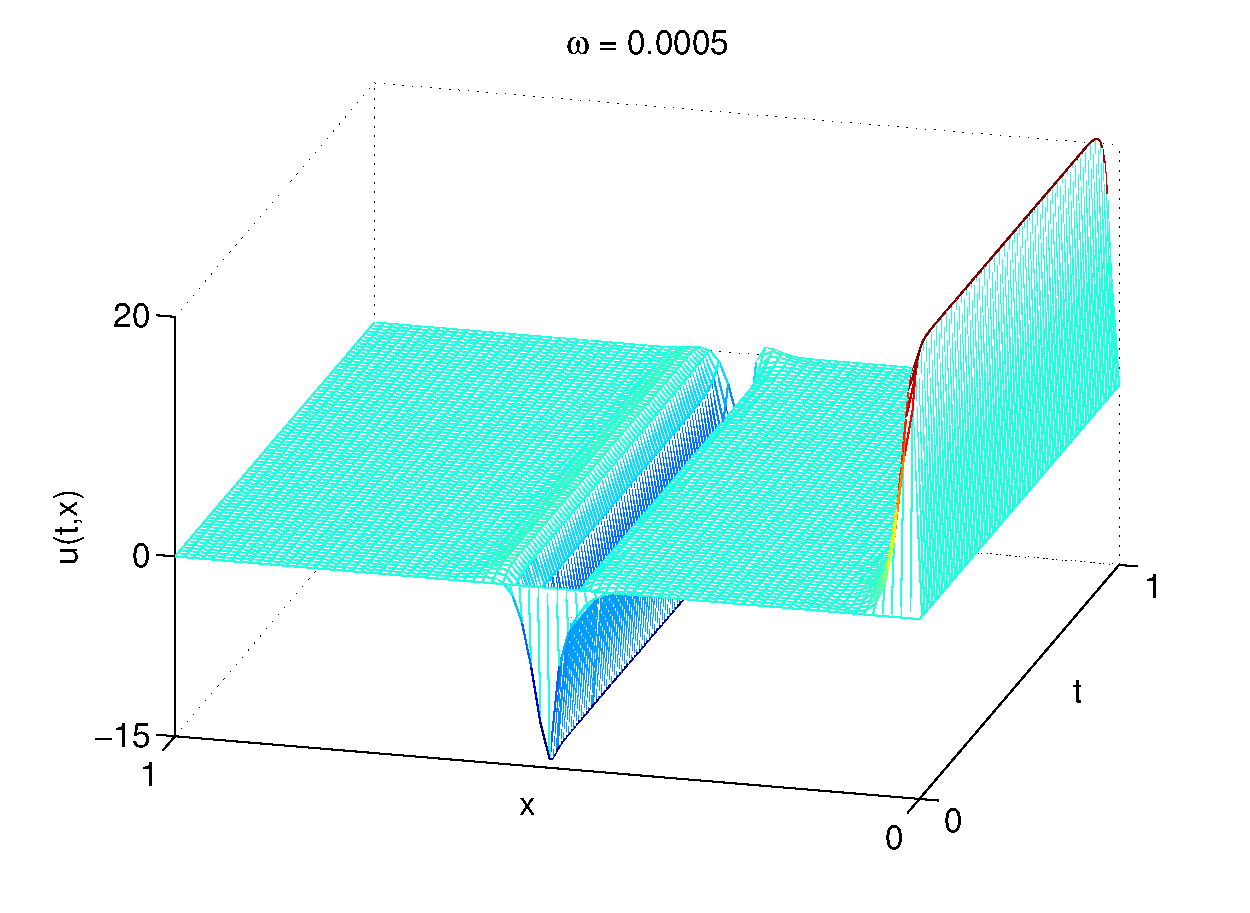
\includegraphics[width=0.33\textwidth]{plots/u_w0005}}\\
\caption{State $y$ and corresponding optimal control $u$ after convergence for different control parameters $\omega = \{0.05, 0.005, 0.0005\}$ .}\label{finalw}
\end{figure}
In Figure \ref{finalw} we see the final state of the optimization for different values of $\omega$ as well as the corresponding optimal control. For the smallest value of $\omega$, we see that the desired state is almost perfectly fitted and, therefore, the control has large values which leads to a large contribution in the cost function but has been compensated by the small value of $\omega$.
\subsection{Numerical results for gradient-based optimization methods}
\label{Num_SPG}
In this section, we present results corresponding to the BFGS and SPG methods as described in Section \ref{BFGS_section} and \ref{SPG_chap}, respectively. In our tests, we used publicly available \textsc{Matlab} implementations that require the cost function and the gradient as input as well as some tolerances and settings. With formula \eqref{minJ_discr} and Algorithm \ref{alg:Adj1_Burgers} we have already given a fully discretized version of the cost function and its gradient and, therefore, the application of both first-order optimization algorithms in straightforward. Here, we only present numerical results of the SPG method because this method allows us to impose bounds on the control $\mathbf{u}$ at all time instance. Accuracy and performance results for all approaches including the BFGS method are presented in Section \ref{numTests}. One can imagine that bounds on the control arise in many engineering application from physical constraints, cf. \cite{SCDA08}.

In Figure \ref{SPGu2}, we present the converged solution of the SPG method when the control is bounded between $-2$ and $2$. Clearly, this affects the corresponding optimal state of Burgers' solution and we can see that the desired state can not be reached with the same accuracy as in the previous examples.
\begin{figure}[H]
\centering
\includegraphics[width=0.8\textwidth]{plots/SPG_u2}
\caption{Optimal state (upper left), desired state (upper right), adjoint state (lower left) and optimal control (lower right) for a bounded control $-2 \leq u \leq 2$ using the SPG Algorithm \ref{alg:SPG}.}\label{SPGu2}
\end{figure}
